\chapter{Groups}
\section{Basic Definitions}
\begin{definition}
Let $S$ be a set. A \textit{binary operation} on $S$ is a map:
\[
* : S \times S \to S
\]
Let $T \subseteq S$ be a subset. We say that the binary operation is \textit{closed} in $T$ if:
\[
\forall a, b \in T, \quad a * b \in T
\]
\end{definition}

\begin{example} Let $S = \mathbb{Z}$. Then the following are binary operations:
\begin{itemize}
    \item $S = \mathbb{Z}, \quad * = +$ (addition)  
    \item $S = \mathbb{Z}, \quad * = \times$ (multiplication)
\end{itemize}
Let 
\[T = \{\text{all even integers}\} \subset \mathbb{Z}.
\] 
For $a, b \in T$, $a+b \in T$ (the sum of two even numbers is even).  
Hence $(T, +)$ is closed in $(S, +)$. Also, if $a,b \in T$, $a \cdot b \in T$ (the product of two even numbers is even).  
Therefore, $(T, \times)$ is also closed in $(S, \times)$.

However, let 
\[
T' = \{\text{all odd integers}\}
\]
Then $(T', +)$ is \textbf{not} closed in $(S, +)$. But for any $(2p+1), (2q+1) \in T'$:
\[
(2p+1)\cdot(2q+1) = 4pq + 2p + 2q + 1
= 2(2pq + p + q) + 1 \in T'
\]
Therefore, $(T', \times)$ is closed in $(S, \times)$.
\end{example}

\begin{example}
\begin{enumerate}
\item Let $S = \mathbb{R}^n$, and $* =$ be the vector addition operation.  
If $W \leq \mathbb{R}^n$ is a vector subspace, then $(W, +)$ is closed in $(\mathbb{R}^n, +)$.

\item Let $S = M_{n\times n}(\mathbb{R})$, and $* =$ multiplication of the ne matrix. Suppose $T = GL_n(\mathbb{R})$ is the subset of all invertible real matrices.  
To check if $T$ is closed in $(S, \times)$:
If $A, B \in T$ (invertible matrices), then  
$A \cdot B$ is invertible since
\[
(AB)^{-1} = B^{-1}A^{-1}
\]
or alternatively:
\[
\det(AB) = \det(A)\det(B) \neq 0
\]
Hence, $T$ is closed in $(S, \times)$.
\end{enumerate}
\end{example}

\begin{definition} [Group] \label{def:group}
A \textbf{group} $G$ is a set along with a binary operation $* : G\times G \to G$ satisfying:
\begin{enumerate}
\item \((a*b)*c = a * (b * c) \quad \forall a,b,c \in G\) \quad (associativity)
\item \(\exists \ e \in G \ \text{such that} \ e * a = a * e = a, \ \forall a \in G\) \quad (identity)
\item \(\forall a \in G, \ \exists b \in G \ \text{s.t.} \ a * b = b * a = e\)  
($b$ is often written as $a^{-1}$, called the inverse of $a$)
\end{enumerate}
\end{definition}
\begin{example}
\begin{itemize}
\item[(a)] $(\mathbb{Z}, +)$ is a group. To see this, note that
\[
\begin{cases}
(a + b) + c = a + (b + c) \quad  \\
0 + a = a + 0 = a \quad \forall a \in \mathbb{Z} \quad (\text{i.e., $e = 0$}) \quad \\
a + (-a) = (-a) + a = 0 \quad (\text{i.e., $a^{-1} = -a$})
\end{cases}
\]
\item[(b)] Similarly $(\mathbb{Q}, +), (\mathbb{R}, +), (\mathbb{C}, +)$ as well as $(\mathbb{Z}_n,+)$ are groups.
\item[(c)] $(\mathbb{Z}, -)$ is \textbf{not} a group, since
\((a - b) - c \neq a - (b - c)\) and \(0 - a \neq a - 0 = a\)
in general, i.e. it is not associative.
\item[(d)] $(\mathbb{Z}, \times)$ is also \textbf{not} a group. Although $(a \times b) \times c = a \times (b \times c)$ is associative, and $a \times 1 = 1 \times a = a$ (so that the identity can be taken as $e = 1$), but there is {\it no} $a \in \mathbb{Z}$ such that
$2 \times a = 1 = e$.)
\item[(e)] $(\mathbb{Q}, \times)$ is \textbf{not} a group. Although now one can take $a = \frac{1}{2}$ such that $2 \times \frac{1}{2} = 1$, yet the element $0 \in \mathbb{Q}$ does not have a multiplicative inverse.
\item[(f)] To resolve the issue, let $\mathbb{Q}^* = \{ q \in \mathbb{Q} \mid q \neq 0 \}$. Then $(\mathbb{Q}^*, \times)$ is a group.
\item[(g)] Similarly, $(\mathbb{R}^*, \times)$ and $(\mathbb{C}^*, \times)$ are groups.
\item[(h)] The set of $2 \times 2$ real matrices, denoted $M_2(\mathbb{R})$, under matrix multiplication $(M_2(\mathbb{R}), \times)$ is \textbf{not} a group, because not all matrices have a multiplicative inverse (namely, singular matrices do not have a multiplicative inverse).
\item[(i)] Let $GL(2, \mathbb{R}) = \{ A \in M_2(\mathbb{R}) \mid \det(A) \neq 0 \}$ be the set of $2 \times 2$ invertible matrices with real entries. Then $(GL(2, \mathbb{R}), \times)$ is a group, known as the general linear group of degree 2 over $\mathbb{R}$.
\end{itemize}
\end{example}

\begin{question}
Given $n \in \mathbb{N}$, for which $a \in \mathbb{Z}$ does $[a]_n$ (the congruence class of $a$ modulo $n$) have a multiplicative inverse in $\mathbb{Z}_n$?
\end{question}

\noindent\textbf{Answer:} 
An element $[a]_n \in \mathbb{Z}_n$ has a multiplicative inverse if and only if $\gcd(a, n) = 1$. 
%{\color{red} add proof using Bezout's theorem. Use \texttt{label} $\backslash \{\ \}$ and \texttt{ref} $\backslash \{\ \}$ to refer to the previously stated theorem}
For instance, when $n=6$, then:
\begin{itemize}
    \item For $a=3$, $\gcd(3, 6) = 3 \neq 1$. Therefore, $[3]_6$ does not have a multiplicative inverse in $\mathbb{Z}_6$.
    \item For $a=5$, $\gcd(5, 6) = 1$. Therefore, $[5]_6$ has a multiplicative inverse in $\mathbb{Z}_6$. Indeed, $[5]_6 \cdot [5]_6 = [25]_6 \equiv [1]_6 \pmod{6}$, so $[5]_6^{-1} = [5]_6$.
\end{itemize}

\begin{remark}
When there is no ambiguity, we often write $ab$ instead of $a \ast b$. Also, for all $m \in \mathbb{Z}$, we denote
    $$a^m := \begin{cases}
        \overbrace{a \ast a \ast \dots \ast a}^{m\ times} &\text{if}\ m > 0 \\
        e &\text{if}\ m = 0 \\
        \overbrace{a^{-1} \ast a^{-1} \ast \dots \ast a^{-1}}^{-m\ times} &\text{if}\ m < 0
    \end{cases}$$

In the case when the operation $\ast$ is the `usual' addition $+$, we call $(G,+)$ {\bf additive group}, and write
$$0 := e, \quad -a := a^{-1}, \quad m \cdot a := a^m.$$
\end{remark}


The order of multiplication matters, namely for $b \in G$, multiplying $a \in G$ on the left or on the right may result in different elements. In the case when they are the same, we have:
\begin{definition}[Abelian Group]
A group $(G, \ast)$ is called \emph{abelian} if its operation is commutative; that is, for all $a, b \in G$, we have $a \ast b = b \ast a$.
\end{definition}

\begin{example}
\begin{itemize}
    \item Examples of abelian groups include: $(\mathbb{Z}, +)$, $(\mathbb{Q}, +)$, $(\mathbb{R}, +)$, $(\mathbb{C}, +)$, and $(\mathbb{Z}_n, +)$.
    \item The group $(GL(2, \mathbb{R}), \times)$ is NOT abelian, as matrix multiplication is generally not commutative.
\end{itemize}
\end{example}

\begin{proposition}
Let $(G, \ast)$ be a group.
\begin{enumerate}
    \item (Uniqueness of Identity) The identity element $e$ in $G$ is unique.
    \item (Uniqueness of Inverses) For each $a \in G$, its inverse $a^{-1}$ is unique.
    \item (Cancellation Laws) For $a, b, c \in G$:
    \begin{itemize}
        \item If $a \ast b = a \ast c$, then $b=c$.
        \item If $b \ast a = c \ast a$, then $b=c$.
    \end{itemize}
\end{enumerate}
\end{proposition}

\section{Cayley Table}

\begin{definition}[Order of a Group]
The \emph{order} of a group $G$, denoted $|G|$, is the number of elements in the group. If $|G| < \infty$, the group is called a \emph{finite group}.
\end{definition}

\begin{definition}[Cayley Table]
For a finite group $(G, \ast)$, a \emph{Cayley table} (or group table) is a square table where the rows and columns are labeled by the elements of the group. The entry in the row corresponding to $a$ and the column corresponding to $b$ is $a \ast b$.
\end{definition}

\begin{example}
The Cayley table for \(\mathbb{Z}_9^*\) is:
\[
\begin{array}{|c||c | c|c|c|c|c|}
\hline
\times & [1]_9 & [2]_9 & [4]_9 & [5]_9 & [7]_9 & [8]_9 \\
\hline \hline
[1]_9 & [1]_9 & [2]_9 & [4]_9 & [5]_9 & [7]_9 & [8]_9 \\
\hline
[2]_9 & [2]_9 & [4]_9 & [8]_9 & [1]_9 & [5]_9 & [7]_9 \\
\hline
[4]_9 & [4]_9 & [8]_9 & [7]_9 & [2]_9 & [1]_9 & [5]_9 \\
\hline
[5]_9 & [5]_9 & [1]_9 & [2]_9 & [7]_9 & [8]_9 & [4]_9 \\
\hline
[7]_9 & [7]_9 & [5]_9 & [1]_9 & [8]_9 & [4]_9 & [2]_9 \\
\hline
[8]_9 & [8]_9 & [7]_9 & [5]_9 & [4]_9 & [2]_9 & [1]_9 \\
\hline
\end{array}
\]
\end{example}


\begin{proposition}
In a Cayley table for a finite group, each element of the group appears exactly once in each row and exactly once in each column. In other words, for all $a \in G$, the sets
$$\{a \ast g\ |\ g \in G\}$$
and 
$$\{g \ast a\ |\ g \in G\}$$
contains all elements of $G$ exactly once, with no repetitions.
\end{proposition}


%\begin{example} Consider a group $G$ with $|G|=4$. For instance, $(\mathbb{Z}_4, +)$ would have a Cayley table where each row and column contains $\{[0]_4, [1]_4, [2]_4, [3]_4\}$ exactly once. \end{example}

\section{Subgroups}

\begin{definition}[Subgroup]
Let $(G, \ast)$ be a group and $H$ be a non-empty subset of $G$. We say that $H$ is a \emph{subgroup} of $G$, denoted $H \le G$, if $(H, \ast)$ is itself a group under the same operation $\ast$ restricted to $H$.
\end{definition}

\begin{proposition}[Subgroup Test]
Let $(G, \ast)$ be a group and $H$ be a non-empty subset of $G$. Then $H$ is a subgroup of $G$ if and only if:
\begin{enumerate}
    \item For all $a, b \in H$, $a \ast b \in H$, i.e. $\ast$ is closed in $H$.
    \item For all $a \in H$, $a^{-1} \in H$ .
\end{enumerate}
Equivalently, one can check the following:
\begin{center}
    For all $a, b \in H$, $a \ast b^{-1} \in H$.
\end{center}
\end{proposition}

\begin{example}
\begin{enumerate}
    \item $(\mathbb{Z}, +) \le (\mathbb{Q}, +) \le (\mathbb{R}, +) \le (\mathbb{C}, +)$.
    \item If $W \leq \mathbb{R}^n$ is a vector subspace, then $(W, +) \leq (\mathbb{R}^n, +)$ is a subgroup.
    \item Let $(G, *) = (\mathbb{Z}, +)$, and $H = \text{all even integers} = 2\mathbb{Z} \subseteq G$. Take $2p, 2q \in H$ ($p, q \in \mathbb{Z}$). Then $2p + 2q = 2(p+q) \in H$ and $-2p = 2(-p) \in H$. Hence, $H \le G$ is a subgroup of $G$.
    More generally, for all $k \in \mathbb{Z}$, $(k\mathbb{Z},+) \le (\mathbb{Z},+)$.
    
    Meanwhile, if $K = \text{all odd integers} \subseteq G$, then $K$ is \textbf{NOT} a subgroup of $G$, since $1, 3 \in K$ but $1 + 3 \notin K$.
    
    \item Let $(G, *) = (GL(n, \mathbb{R}), \cdot)$, and 
    $$SL(n, \mathbb{R}) := \{ A \in G \mid \det(A) = 1 \}$$ 
    Then $SL(n,\mathbb{R}) \leq GL(n, \mathbb{R})$:
    \begin{itemize} 
    \item For all $A, B \in SL(n, \mathbb{R})$,  $\det(AB) = \det(A) \cdot \det(B) = 1 \cdot 1 = 1$. Therefore, $AB \in SL(n, \mathbb{R})$ 
    for all $A, B \in SL(n, \mathbb{R})$ 
    \item For all $A \in SL(n, \mathbb{R})$, $\det(A^{-1}) = \frac{1}{\det(A)} = \frac{1}{1} = 1$. Therefore, $A^{-1} \in SL(n, \mathbb{R})$ as well.
    \end{itemize}
    \item Let $(G, *) = (\mathbb{Z}_8, +)$. Then $ H = \{0, 4\}$ is a subgroup of $G$, while $K = \{0, 3\}$ is \textbf{NOT} a subgroup.
\end{enumerate}
\end{example}

\begin{definition}
Let $(G, *)$ be a group. Then:
    \begin{enumerate}
        \item $(G, *) \le (G, *)$ is a subgroup of $G$. We say all $H \le G$ satisfying $H \neq G$ a {\bf proper subgroup} of $G$.
        \item $\{e\} \le G$ is a subgroup. We say all $H \le G$ with $H \neq \{e\}$ a {\bf nontrivial subgroup} of $G$.
    \end{enumerate}
\end{definition}


\section{Cyclic Groups}

\begin{definition}[Cyclic Subgroup]
Let $(G, *)$ be a group. A {\bf cyclic subgroup} generated by $g \in G$ is the subgroup $$\langle g \rangle := \{ g^m \mid m \in \mathbb{Z} \}.$$
\end{definition}
\noindent (Exercise: Check $\langle g \rangle \le G$ is a subgroup of $G$, i.e.: for any
$g^a, g^b \in \langle g \rangle \quad \begin{cases} g^a * g^b \in \langle g \rangle \\ (g^a)^{-1} \in \langle g \rangle \end{cases}$.)

\begin{example}
Here are some examples of cyclic subgroups:
\begin{enumerate}
    \item Let $(G, *) = (\mathbb{Z}, +)$, then 
    $$\langle 2 \rangle = \{ 2, 2+2, 2+2+2, \dots, 0, (-2), (-2)+(-2), (-2)+(-2)+(-2), \dots \} = 2\mathbb{Z}.$$
    
    \item Let $(G, *) = (GL(2, \mathbb{R}), \cdot)$, then    $$\left\langle \begin{pmatrix} 1 & 1 \\ 0 & 1 \end{pmatrix} \right\rangle = \left\{ \begin{pmatrix} 1 & 1 \\ 0 & 1 \end{pmatrix}^m \middle| m \in \mathbb{Z} \right\} = \left\{ \begin{pmatrix} 1 & m \\ 0 & 1 \end{pmatrix} \middle| m \in \mathbb{Z} \right\}.$$ 
    ( Check: $\begin{pmatrix} 1 & a \\ 0 & 1 \end{pmatrix} \cdot \begin{pmatrix} 1 & b \\ 0 & 1 \end{pmatrix} = \begin{pmatrix} 1 & a+b \\ 0 & 1 \end{pmatrix}$ )
    
    \item Let $(G, *) = (\mathbb{Z}_8, +)$, then
    $$\langle 2 \rangle = \{ 0, 2, 4, 6, \dots \} = \{ 0, 2, 4, 6 \}$$
    $$\langle 3 \rangle = \{ 0, 3, 6, 9, 12, 15, 18, 21, 24, \dots \} = \{ 0, 3, 6, 1, 4, 7, 2, 5, 0, \dots \} = G$$
\end{enumerate}
\end{example}

\begin{definition}[Cyclic Group]
Let $(G, *)$ be a group. We say $G$ is \textbf{cyclic} if there is $g \in G$ such that $\langle g \rangle = G$.
\end{definition}


\begin{example}
\begin{itemize}
    \item $(G, *) = (\mathbb{Z}, +)$ is cyclic, since $G = \langle 1 \rangle$.
    \item $(G, *) = (\mathbb{Z}_8, +)$ is cyclic, since $G = \langle 3 \rangle = \langle 1 \rangle$.
    \item $(G, *) = (GL(2, \mathbb{R}), \cdot)$ is \textbf{NOT} cyclic, since for all $H = \langle g \rangle$, $H$ is countable but $G$ is uncountable. 
    Hence, $H$ can never be equal to $G$.
    
    \item $(G, *) = (\mathbb{Z}_8^*, \cdot) = \{ 1, 3, 5, 7 \}$. Then the cyclic subgroups of $G$ are: \\
    $\langle 1 \rangle = \{ 1 \}$,\\ 
    $\langle 3 \rangle = \{ 3^0=1, 3^1=3, 3^2=1, 3^3=3, \dots \} = \{ 1, 3 \}$;\\
    $\langle 5 \rangle = \{ 1, 5 \}$; \\
    $\langle 7 \rangle = \{ 1, 7 \}$. 
    
    Note that none of them is equal to $G$. So $G$ is \textbf{not} cyclic.
\end{itemize}
\end{example}

\noindent \textbf{Question:} $(G, *)$ group, $H = \langle g \rangle$. What's the order of $H$? For instance, if $G = (\mathbb{Z}_8, +)$, then $ |\langle [2] \rangle| = 4, \ |\langle [3] \rangle| = 8, \ |\langle [4] \rangle| = 2$.
\begin{definition}[Order] 
Let $g \in G$. The \textit{order} of $g$ is equal to the smallest positive integer $k$ such that $g^k = e$. If no such $k$ exists, then we say the order of $g$ is $\infty$.
\end{definition}

\begin{proposition} \label{prop:ordg}
If $\mathrm{ord}(g) = k$, then $|\langle g \rangle| = k$.
\end{proposition}

\begin{example}
\begin{itemize}
    \item $(G, *) = (\mathbb{Z}_8, +)$. $\text{ord}([2]) = 4$ since $$[2]=[2], [2]+[2]=[4], [2]+[2]+[2]=[6], [2]+[2]+[2]+[2]=[8] = [0].$$
    Also, $\text{ord}([3]) = 8$, since 
    $$1 \cdot [3]=[3],\ 2 \cdot [3] =[6],\ 3 \cdot [3]=[9] = [1],\ 4 \cdot [3]=[12] = [4],$$ $$5 \cdot [3]=[15] = [7],\ 6 \cdot [3]=[18] = [2],\ 7 \cdot [3]=[21] = [5],\ 8 \cdot [3] =[24] = [0].$$
    \item Let $(G, *) = (GL(2, \mathbb{R}), \cdot)$. Then 
    $\text{ord}\left( \begin{pmatrix} 1 & 1 \\ 0 & 1 \end{pmatrix} \right) = \infty$, since $$\begin{pmatrix} 1 & m \\ 0 & 1 \end{pmatrix} = \begin{pmatrix} 1 & 1 \\ 0 & 1 \end{pmatrix}^m \neq \begin{pmatrix} 1 & 0 \\ 0 & 1 \end{pmatrix} \quad \forall m \in \mathbb{N}.$$
\end{itemize}
\end{example}
\vspace{1em}
\begin{remark} 
If $|G| < \infty$ is finite, then $\langle g \rangle \le G$ is a finite subgroup with $|\langle g \rangle| \le |G|$. Indeed, all $H \le G$ has $|H| \mid |G|$ (see Section \ref{sec:Lagrange} - Lagrange's Theorem below). \\
e.g.: If $|G|=12$, then there is \textbf{NO} $H \le G$ with $|H|=8$, can only be $1, 2, 3, 4, 6, 12$. \\
Therefore, $\text{ord}(g) \mid |G|$ (take $H = \langle g \rangle$).
\end{remark}

\vspace{1em}
\section{More examples of Groups}
\subsection*{Permutation group / Symmetric group $S_n$}


\begin{definition} 
A \textit{permutation} of $X_n = \{1, 2, \dots, n\}$ is a bijection $\sigma : X_n \to X_n$. \\
\end{definition}
For example, when $n=3$, $\sigma(1)=2, \sigma(2)=3, \sigma(3)=1$ is a permutation.

\begin{definition} 
The \textbf{symmetric / permutation group} of $n$ elements is the collection of all permutations $\sigma : X_n \to X_n$.
\[ S_n := \{ \sigma : X_n \to X_n \mid \sigma \text{ is bijective} \} \]
\end{definition}
For instance, when $n = 3$, one has:
\begin{center}
\usetikzlibrary{arrows.meta, bending}
\begin{tikzpicture}[
    ball/.style={circle, draw=black, thick, minimum size=6mm, font=\small},
    arrow/.style={-{Stealth}, thick, blue!70!black, shorten >=2pt, shorten <=2pt},
    scale=0.8
]

    \newcommand{\drawpermutation}[7]{
        \begin{scope}[shift={(#2, #3)}]
            % Top Row
            \foreach \i in {1,2,3} {
                \node[ball] (T\i) at (\i*1.2, 2) {\i};
            }
            % Bottom Row
            \foreach \i in {1,2,3} {
                \node[ball] (B\i) at (\i*1.2, 0) {\i};
            }
            % Arrows
            \draw[arrow] (T1) -- (B#4);
            \draw[arrow] (T2) -- (B#5);
            \draw[arrow] (T3) -- (B#6);
            % Label
            \node at (2.4, -1) {\textbf{#7}};
        \end{scope}
    }

    % --- ROW 1: Identity and 3-Cycles ---
    \drawpermutation{id}{0}{0}{1}{2}{3}{}
    \drawpermutation{c123}{5}{0}{2}{3}{1}{}
    \drawpermutation{c132}{10}{0}{3}{1}{2}{}

    % --- ROW 2: Transpositions (Swaps) ---
    \drawpermutation{t12}{0}{-5}{2}{1}{3}{}
    \drawpermutation{t23}{5}{-5}{1}{3}{2}{}
    \drawpermutation{t13}{10}{-5}{3}{2}{1}{}
\end{tikzpicture}
\end{center}
Hence $|S_3|=6$. More generally, 
$$|S_n| = n \cdot (n-1) \cdots 1 = n!.$$
\begin{proposition} 
$(S_n, \circ)$ is a group, where $\circ$ is the composition of functions. 
\end{proposition}
\begin{proof} We need to show that the three axioms of groups hold for $(S_n, \circ)$:
\begin{enumerate}
    \item $(\sigma_1 \circ \sigma_2) \circ \sigma_3 = \sigma_1 \circ (\sigma_2 \circ \sigma_3)$ is true, since composition of functions $\circ$ is associative.
    \item Take $e = \text{id} : X_n \to X_n$, $e(i) := i$ for all $1 \leq i \leq n$. Then $\sigma \circ e = e \circ \sigma = \sigma$.
    \item Since $\sigma$ is bijective, then $\sigma^{-1} : X_n \to X_n$ exists with $\sigma \circ \sigma^{-1} = \sigma^{-1} \circ \sigma = e$.
\end{enumerate}
\end{proof}


\begin{remark} \label{rmk-symmetrysn}
Groups are often used to study "symmetry" of objects. For example, $S_n$ can be used to study symmetry of $n$ identical objects. Here is an example of $n=4$:
\begin{center}
\begin{tikzpicture}[
    ball/.style={circle, draw=black, thick, minimum size=1cm, fill=blue!20},
    arrow/.style={-{Stealth}, thick, shorten >=2pt, shorten <=2pt, gray!80}
]

    % --- Top Row (Original Positions) ---
    \node[ball] (T1) at (0, 3) {};
    \node[ball] (T2) at (2, 3) {};
    \node[ball] (T3) at (4, 3) {};
    \node[ball] (T4) at (6, 3) {};
    
    \node[anchor=west] at (7, 3) {Original};

    % --- Bottom Row (Permuted Positions) ---
    \node[ball] (B1) at (0, 0) {};
    \node[ball] (B2) at (2, 0) {};
    \node[ball] (B3) at (4, 0) {};
    \node[ball] (B4) at (6, 0) {};

    \node[anchor=west] at (7, 0) {Permuted};

    % --- Permutation Arrows ---
    % 1 moves to the 3rd spot
    \draw[arrow] (T1) -- (B3);
    % 2 moves to the 1st spot
    \draw[arrow] (T2) -- (B1);
    % 3 moves to the 4th spot
    \draw[arrow] (T3) -- (B4);
    % 4 moves to the 2nd spot
    \draw[arrow] (T4) -- (B2);

\end{tikzpicture}
\end{center}
Although we have carried out a permutation $1 \mapsto 3$, $2 \mapsto 1$, $3 \mapsto 4$, $4 \mapsto 2$, one cannot tell the difference of the objects before and after permutation. 

As another example, to describe (some) symmetries of $\mathbb{R}^n$, we have: 
$$GL(n, \mathbb{R}) = \{ A : \mathbb{R}^n \to \mathbb{R}^n \mid A \text{ is a bijective linear transformation} \}$$
which can be seen as a certain kind of `permutation' on the points in $\mathbb{R}^n$.
\end{remark}

\subsection*{Calculations on $S_n$}
We use cycle notations to denote elements of $S_n$. 

\begin{definition}
A permutation $\sigma \in S_n$ is called a \textbf{$k$-cycle} (or a cycle of length $k$) if there exists a set of $k$ distinct elements $\{a_1, a_2, \dots, a_k\} \subseteq \{1, 2, \dots, n\}$ such that:
\[
\sigma(a_1) = a_2, \quad \sigma(a_2) = a_3, \quad \dots, \quad \sigma(a_{k-1}) = a_k, \quad \sigma(a_k) = a_1
\]
and $\sigma(i) = i$ for all $i \notin \{a_1, a_2, \dots, a_k\}$.

As an example, the element $\sigma \in S_4$ in Remark \ref{rmk-symmetrysn} is a $4$-cycle $\sigma =(1\ 3\ 4\ 2)$.
\end{definition} 

Note that every $\sigma \in S_n$ can be expressed as a product of {\bf disjoint} cycles (possibly of different lengths):
$$\sigma = (a_1 \dots a_k) (b_1 \dots b_l) \cdots (c_1 \dots c_m) := (a_1 \dots a_k) \circ (b_1 \dots b_l) \circ \cdots \circ(c_1 \dots c_m).$$
where the sets $\{a_1, \dots , a_k\}$, $\{b_1, \dots , b_l\}$, $\cdots$, $\{c_1, \dots , c_m\}$ are disjoint subsets of $X_n$. For instance, in $S_8$, the permutation
\begin{center}
$1 \to 3$,\quad $2 \to 5$,\quad $3 \to 1$,\quad $4 \to 6$,\quad $5 \to 2$,\quad $6 \to 8$,\quad $7 \to 7$,\quad $8 \to 4$ 
\vspace{3mm}
\\
\begin{tikzpicture}[
    ball/.style={circle, draw=black, thick, minimum size=0.8cm, fill=white},
    arrow/.style={-{Stealth}, thick, shorten >=2pt, shorten <=2pt}
]

    % --- Nodes for Top Row (Original Indices) ---
    \foreach \i in {1,...,8} {
        \node[ball] (T\i) at (\i*1.5, 3) {\i};
    }
    \node[anchor=west, font=\small\bfseries] at (12.5, 3) {Index $i$};

    % --- Nodes for Bottom Row (Values) ---
    \foreach \i in {1,...,8} {
        \node[ball] (B\i) at (\i*1.5, 0) {\i};
    }
    \node[anchor=west, font=\small\bfseries] at (12.5, 0) {Image $\sigma(i)$};

    % --- Permutation Arrows (Color-coded by Cycle) ---
    
    % Cycle (1 3) - Red
    \draw[arrow, red] (T1) -- (B3);
    \draw[arrow, red] (T3) -- (B1);

    % Cycle (2 5) - Blue
    \draw[arrow, blue] (T2) -- (B5);
    \draw[arrow, blue] (T5) -- (B2);

    % Cycle (4 6 8) - Teal
    \draw[arrow, teal] (T4) -- (B6);
    \draw[arrow, teal] (T6) -- (B8);
    \draw[arrow, teal] (T8) -- (B4);

    % Cycle (7) - Orange
    \draw[arrow, orange] (T7) -- (B7);
\end{tikzpicture}
\end{center}
can be split into:
\begin{itemize}
    \item $1 \to 3$ and $3 \to 1$. This gives the cycle $(1 \, 3)$.
    \item $2 \to 5$ and $5 \to 2$. This gives the cycle $(2 \, 5)$.
    \item $4 \to 6$, $6 \to 8$, and $8 \to 4$. This gives the cycle $(4 \, 6 \, 8)$.
    \item $7 \to 7$. This is a fixed point, giving the 1-cycle $(7)$.
\end{itemize}
Therefore,
\[
\sigma = (1 \, 3)(2 \, 5)(4 \, 6 \, 8)(7) := (1 \, 3) \circ (2 \, 5) \circ (4 \, 6 \, 8) \circ (7)
\]

Here are some examples in calculating products in $S_n$:
\begin{example}
Let $\sigma = (1\,2\,3)$, $\tau = (1\,3\,4\,2)(7\,6)$ in $S_7$. Then:
\begin{itemize}
    \item $\sigma\tau = (1\,2\,3)(1\,3\,4\,2)(7\,6) = (1)(2)(3\,4)(7\,6) = (3\,4)(6\,7)$.
    \item $\tau\sigma = (1\,3\,4\,2)(7\,6)(1\,2\,3) = (1)(2\,4)(3)(6\,7) = (2\,4)(6\,7)$.
\end{itemize}
Therefore, 
\begin{center}
{\bf $\sigma \circ \tau \neq \tau \circ \sigma$ in general, i.e. $S_n$ is not abelian for $n \geq 3$.} 
\end{center}
\end{example}
\vspace{1em}
\begin{remark}
\begin{itemize}
    \item From now on, we'll express $\sigma \in S_n$ using (disjoint) product of $k$-cycles.
    \item If $\alpha$ and $\beta$ are $k$-cycles with disjoint entries, then $\alpha\beta = \beta\alpha$. \\
    (e.g.: $\alpha = (1\,3\,2)$, $\beta = (4\,7) \Rightarrow \alpha\beta = (1\,3\,2)(4\,7) = (4\,7)(1\,3\,2) = \beta\alpha$). \\
    Otherwise, $\alpha\beta \neq \beta\alpha$ in general.
    \item The inverse of a $k$-cycle is given by:
    \[ (i_1\,i_2 \dots i_k)^{-1} = (i_1\,i_k\,i_{k-1} \dots i_2) \]
    \item More generally, for any $\sigma \in S_n$, $\sigma = (i_1 \dots i_k)(j_1 \dots j_\ell) \dots (m_1 \dots m_p)$ where the cycles are disjoint, then:
    \[ \sigma^{-1} = (i_1\,i_k \dots i_2)(j_1\,j_\ell \dots j_2) \dots (m_1\,m_p \dots m_2) \]
\end{itemize}
\end{remark}

\subsection*{Alternating Group $A_n$}
\begin{definition}[Transposition]
A 2-cycle $\tau = (i\,j) \in S_n$ is called a \textbf{transposition}.
\end{definition}
\vspace{1em}
\begin{proposition}
Every $\sigma \in S_n$ can be expressed as a product of (NOT necessarily disjoint) transpositions.
\end{proposition}

\begin{proof}
$\sigma = (i_1 \dots i_k)(j_1 \dots j_\ell) \dots (m_1 \dots m_p)$ with each $i, j, \dots, m$ cycles are disjoint. Then for $(i_1 \dots i_k)$:
\[ (i_1 \dots i_k) = (i_1\,i_k)(i_1\,i_{k-1}) \dots (i_1\,i_3)(i_1\,i_2) \]
Do the same for $(j_1 \dots j_\ell), \dots, (m_1 \dots m_p)$. Then we're done. \end{proof}

\begin{remark}
The expression of $\sigma \in S_n$ into product of transpositions is \textbf{NOT} unique. For example, $$\sigma = (2\,3) = (2\,3)(2\,3)(2\,3) = (1\,2)(2\,3)(1\,3).$$ 
But the number of transpositions in each expression of $\sigma$ is always \textbf{even} or \textbf{odd}, as we will see below.
\end{remark}

\begin{lemma} \label{lem-idiseven}
If $e = \tau_1 \cdots \tau_k$, where each $\tau_i$ is a transposition. Then $k \equiv 0 \pmod 2$ is even.
\end{lemma}

\begin{proof}
Apply induction on $k$, that is,
\begin{center}
If $e = \tau_1 \cdots \tau_k$, then $k$ is even. \quad \quad (*)
\end{center}
The case of $k=0$ is trivial. Also, it is obvious that the $k \neq 1$, since $e$ cannot be equal to any single transposition $\tau$. So (*) holds for $k=1$. 

Now suppose by induction hypothesis that (*) holds for all expressions of $e = \tau'_1 \cdots \tau'_{k'}$ for $k' \le m$. Consider 
$$e = \tau_1 \cdots \tau_m \tau_{m+1},$$ 
an expression of $e$ with $(m+1)$ transpositions. Let $\tau_{m+1} = (a\,b)$, Then:

\textbf{Case 1:} $\tau_m = (a\,b)$. In this case, $e = \tau_1 \cdots \tau_{m-1}(a\,b)(a\,b) = \tau_1 \cdots \tau_{m-1}$. By induction, $m-1 \equiv 0 \pmod 2$. Hence, $m+1 \equiv 0 \pmod 2$ is even.

\textbf{Case 2:} $\tau_m \neq (a\,b)$. Then $\tau_m = $
$\begin{cases} 
(a\,c) & c \neq b\\
(b\,d) & d \neq a \\
(i\,j)(a\,b) & \{i,j\} \cap \{a,b\} = \emptyset
\end{cases}$. Then one has
$$\tau_m \tau_{m+1} = 
\begin{cases} 
(a\,c)(a\,b) = (a\,b)(b\,c) \\
(b\,d)(a\,b) = (a\,d)(d\,b) \\
(i\,j)(a\,b) = (a\,b)(i\,j) 
\end{cases}$$ 
(where the right hand side in the new expression ($(b\ c)$, $(d\ b)$, $(i\ j)$) have no "$a$"s). Therefore,
$$e = \tau_1 \cdots \tau_{m-1} \tau_m \tau_{m+1} = \tau_1 \cdots \tau_{m-1} (a\,\star)(\ast\,\ast).$$
where $\ast \neq a$. 

Continue the same argument on  $\tau_1 \dots \tau_{m-1}(a\,*)$. If $\tau_{m-1} = (a\,*)$, then $\tau_{m-1}(a\,*)$ goes away. Then one can apply induction as in Case 1 and get the same conclusion. Otherwise, $\tau_{m-1} \neq (a\,*)$, then we use Case 2 to move one more step to the left and get: 
$$e = \tau_1 \cdots \tau_{m-2} (a\, \square)(\ast \,\ast)(\ast\,\ast)$$ 
with $\ast \neq a$. 

We keep moving $a$ to the left, and claim that Case 1 must occur somewhere, so that we can apply the induction argument to conclude $m+1$ is even. Otherwise, we can keep applying Case 2 to `push' $a$ to the leftmost position, and get
$$e = (a\,\triangle) (*\,*) \cdots (*\,*)$$ 
with $\ast \neq a$. But this \textbf{cannot} happen, since the expression on right-hand-side permutes $a \to \triangle$ (note that $(a\ \triangle)$ is the only transposition on the right that moves $a$), which contradicts that fact that it is the identity element. 
\end{proof}

\begin{proposition}
Let $\sigma = \tau_1 \cdots \tau_k = \tau'_1 \cdots \tau'_\ell$ be two expressions of $\sigma$ as product of transpositions. Then $k \equiv \ell \pmod 2$.
\end{proposition}

\begin{proof}
$$e = \sigma^{-1} \sigma = (\tau_1 \cdots \tau_k)^{-1} (\tau'_1 \cdots \tau'_\ell) = \tau_k^{-1} \cdots \tau_1^{-1} \tau'_1 \cdots \tau'_\ell = \tau_k \cdots \tau_1 \tau'_1 \cdots \tau'_\ell.$$
Then by Lemma \ref{lem-idiseven}, $k + \ell \equiv 0 \pmod 2$.
\end{proof}

\begin{definition}
$\sigma \in S_n$ is called an \textbf{even / odd permutation} if $\sigma$ is a product of an even / odd number of transpositions.
\end{definition}

\begin{definition}[Alternating Group]
The \textbf{alternating group} $A_n$ is the subgroup of $S_n$ given by:
\[ A_n := \{ \sigma \in S_n \mid \sigma \text{ is even} \} \]
\end{definition}
\noindent (Check: $A_n \le S_n$. Also, is the set $\{ \sigma \in S_n \mid \sigma \text{ is odd} \}$ a subgroup?)

\begin{proposition}
$|A_n| = \frac{1}{2} |S_n| = \frac{n!}{2}$
\end{proposition}

\begin{proof}
Let $\tau \in S_n$ be a transposition and define $f : A_n \to \{ \sigma \in S_n \mid \sigma \text{ odd} \}$ by:
$$f(\sigma) := \sigma \tau.$$ 
Note that $f$ is bijective with $f^{-1} = f$. Hence, $|A_n| = |\{ \sigma \in S_n \mid \sigma \text{ odd} \}|$. 

Since $A_n \cap \{ \sigma \in S_n \mid \sigma \text{ odd} \} = \emptyset$, and
$A_n \sqcup \{ \sigma \in S_n \mid \sigma \text{ odd} \} = S_n$, therefore $$|A_n| = \frac{|S_n|}{2} = \frac{n!}{2}.$$ 
\end{proof}

\begin{example}

\begin{enumerate}
    \item $A_4$ is the group of ``symmetries of a tetrahedron''.

\begin{center}
\usetikzlibrary{arrows.meta, calc}
\begin{tikzpicture}[line join=round, line cap=round, scale=2]
    % Style for vertices
    \tikzset{vertex/.style={circle, fill=white, draw=black, inner sep=1pt, font=\small}}
    
    % --- DIAGRAM 1: 120-degree rotation axis ---
    \begin{scope}[shift={(0,0)}]
        % Coordinates
        \coordinate (V1) at (0, 1.5, 0);
        \coordinate (V2) at (-0.8, 0, 0.5);
        \coordinate (V3) at (0.8, 0, 0.5);
        \coordinate (V4) at (0, 0, -0.8);

        % Hidden edge
        \draw[dashed, gray] (V2) -- (V4);
        
        % Axis of rotation (Through Vertex 1 and center of opposite face)
        \draw[thick, red, dashed] (0, 1.9, 0) -- (0, -0.5, 0);
        
        % Rotation indicator arc at the top
        \draw[red, -{Stealth}] (0.2, 1.7) arc (0:270:0.2 and 0.08);
        \node[red, right, font=\tiny] at (0.2, 1.75) {$120^\circ$};

        % Solid edges
        \draw[thick] (V1) -- (V2) -- (V3) -- (V1);
        \draw[thick] (V1) -- (V4) -- (V3);

        % Vertices
        \node[vertex] at (V1) {1};
        \node[vertex] at (V2) {2};
        \node[vertex] at (V3) {3};
        \node[vertex] at (V4) {4};

        \node at (0, -0.8) {Rotation $(2\,3\,4)$};
    \end{scope}

    % --- DIAGRAM 2: 180-degree rotation axis ---
    \begin{scope}[shift={(2.5,0)}]
        % Coordinates
        \coordinate (V1) at (0, 1.5, 0);
        \coordinate (V2) at (-0.8, 0, 0.5);
        \coordinate (V3) at (0.8, 0, 0.5);
        \coordinate (V4) at (0, 0, -0.8);
        
        % Midpoints for the axis (edges 1-3 and 2-4)
        \coordinate (M13) at ($(V1)!0.5!(V3)$);
        \coordinate (M24) at ($(V2)!0.5!(V4)$);

        % Hidden edges
        \draw[dashed, gray] (V2) -- (V4);
        \draw[dashed, gray] (V1) -- (V4);
        
        % Axis of rotation (Through midpoints of opposite edges)
        \draw[thick, red, dashed] ($(M13)!-0.6!(M24)$)--($(M24)!-0.6!(M13)$);
        
        % Rotation indicator arc around the axis
        % (Placed near the top midpoint)
        \draw[red, -{Stealth}] ($(M13)+(0.1, 0.2)$ ) arc (0:270:0.15 and 0.06);
        \node[red, right, font=\tiny] at ($(M13)+(0.1, 0.25)$) {$180^\circ$};

        % Solid edges
        \draw[thick] (V1) -- (V2) -- (V3) -- (V1);
        \draw[thick] (V4) -- (V3);

        % Vertices
        \node[vertex] at (V1) {1};
        \node[vertex] at (V2) {2};
        \node[vertex] at (V3) {3};
        \node[vertex] at (V4) {4};

        \node at (0, -0.8) {Rotation $(1\,3)(2\,4)$};
    \end{scope}

\end{tikzpicture}
\end{center}    
    
    
    \begin{itemize}
        \item A rotation of the tetrahedron corresponds to a permutation of its 4 vertices. For example, a $120^\circ$ rotation about a vertex fixies one vertex and cyclically permutes the other three:
        \[ (2\,3\,4) = (2\,4)(2\,3) \in A_4 \]
        \item A $180^\circ$ rotation about the midpoints of opposite edges corresponds to:
        \[ (1\,3)(2\,4) \in A_4 \]
    \end{itemize}

    
    \item If we allow reflections (not just rotations), we get the full symmetric group, e.g. $(2\,4) \in S_4 \setminus A_4$ comes from the reflection:
\begin{center}
\begin{tikzpicture}[line join=round, line cap=round, scale=2]
    % Style for vertices
    \tikzset{vertex/.style={circle, fill=white, draw=black, inner sep=1pt, font=\small}}
    
    % Coordinates (Consistent with previous diagrams)
    \coordinate (V1) at (0, 1.5, 0);
    \coordinate (V2) at (-0.8, 0, 0.5);
    \coordinate (V3) at (0.8, 0, 0.5);
    \coordinate (V4) at (0, 0, -0.8);
    
    % Midpoint of the edge being swapped (2-4)
    \coordinate (M24) at ($(V2)!0.5!(V4)$);

    % --- 1. Draw back/hidden parts ---
    \draw[dashed, gray] (V2) -- (V4);
    \draw[dashed, gray] (V1) -- (V4);

    % --- 2. Draw the Reflection Plane ---
    % The plane passes through V1, V3, and the midpoint of V2-V4
    \fill[red, opacity=0.2] (V1) -- (V3) -- (M24) -- cycle;
    \draw[red, thick, dashed] (V1) -- (M24);
    \draw[red, thick] (V1) -- (V3);
    \draw[red, thick, dashed] (V3) -- (M24);

    % --- 3. Draw the solid edges of the tetrahedron ---
    \draw[thick] (V1) -- (V2) -- (V3) -- cycle;
    \draw[thick] (V3) -- (V4);

    % --- 4. Vertices ---
    \node[vertex] at (V1) {1};
    \node[vertex] at (V2) {2};
    \node[vertex] at (V3) {3};
    \node[vertex] at (V4) {4};

    % Label
    \node at (0, -0.8) {Reflection $(2\,4)$};
    
    % Small text explaining the plane
    \node[red, font=\tiny, align=center] at (1.2, 1.2) {Reflection Plane \\ fixes 1 and 3};

\end{tikzpicture}
\end{center}
    
    
    \item \textbf{Galois Theory}: $A_5$ is a simple group (we will define simple group later). This is a purely group theoretic observation, but it is used by Galois to showing that a general quintic (degree-$5$) equation {\bf cannot} be solved using radicals, i.e. $+, \times, \frac{*}{*}, \sqrt[k]{*}$.
\end{enumerate}
\end{example}
\subsection*{Dihedral Groups $D_n$}
We begin by giving an informal definition of the dihedral group $D_n$: 
\begin{center}
The dihedral group $D_n$ describes the rotational and reflectional symmetries of a regular $n$-gon. Here are the pictures for $n = 3, 4, 5$:
\end{center}

\begin{tikzpicture}[scale=1.2,
    polygon/.style={thick},
    axis/.style={blue,dashed,thick},
    rot/.style={red,thick,-{Stealth[length=3mm]}}
]

% =========================
% Regular 3-gon (Triangle)
% =========================
\begin{scope}[shift={(0,0)}]
    \node at (0,2.3) {\textbf{Regular 3-gon}};
    
    % vertices
    \foreach \i in {0,1,2}
        \coordinate (T\i) at ({90+120*\i}:1.2);
    
    % polygon
    \draw[polygon] (T0)--(T1)--(T2)--cycle;
    
    % reflection axes (FULL lines)
    \foreach \i in {0,1,2}
        \draw[axis]
            ({90+120*\i}:1.8) -- ({90+120*\i+180}:1.8);
    
    % rotation arrow
    \draw[rot] (0.6,0) arc (0:110:0.6);
    \node[red] at (0.9,0.5) {$120^\circ$};
\end{scope}

% =========================
% Regular 4-gon (Square)
% =========================
\begin{scope}[shift={(5,0)}]
    \node at (0,2.3) {\textbf{Regular 4-gon}};
    
    % vertices
    \foreach \i in {0,1,2,3}
        \coordinate (S\i) at ({45+90*\i}:1.2);
    
    % polygon
    \draw[polygon] (S0)--(S1)--(S2)--(S3)--cycle;
    
    % reflection axes
    \draw[axis] (-1.8,0)--(1.8,0);
    \draw[axis] (0,-1.8)--(0,1.8);
    \draw[axis] (-1.6,-1.6)--(1.6,1.6);
    \draw[axis] (-1.6,1.6)--(1.6,-1.6);
    
    % rotation arrow
    \draw[rot] (0.6,0) arc (0:90:0.6);
    \node[red] at (0.9,0.4) {$90^\circ$};
\end{scope}

% =========================
% Regular 5-gon (Pentagon)
% =========================
\begin{scope}[shift={(10,0)}]
    \node at (0,2.3) {\textbf{Regular 5-gon}};
    
    % vertices
    \foreach \i in {0,...,4}
        \coordinate (P\i) at ({90+72*\i}:1.2);
    
    % polygon
    \draw[polygon]
        (P0)--(P1)--(P2)--(P3)--(P4)--cycle;
    
    % reflection axes (FULL lines)
    \foreach \i in {0,...,4}
        \draw[axis]
            ({90+72*\i}:1.8) -- ({90+72*\i+180}:1.8);
    
    % rotation arrow
    \draw[rot] (0.6,0) arc (0:70:0.6);
    \node[red] at (0.95,0.35) {$72^\circ$};
\end{scope}

\end{tikzpicture}

For example, when $n=3$, $D_3$ describes the symmetries of an equilateral triangle:
    \begin{itemize}
        \item Rotations: $e$, $\sigma_{120^\circ}$, $\sigma_{240^\circ}$.
        \item Reflections: 3 axes of symmetry, each fixing one vertex and swapping the other two.
    \end{itemize}
Hence, $D_3$ has 6 elements.
As for $n=4$, $D_4$ describes the symmetries of a square, namely:
    \begin{itemize}
        \item There are 4 rotations $e$, $\sigma_{90^\circ}$, $\sigma_{180^\circ}$, $\sigma_{270^\circ}$
        \item There are also 4 reflections - 2 reflections on along the diagonals, and 2 reflections along the midpoints of the parallel sides.
    \end{itemize}
Hence, $|D_4| = 8$, and more generally, $|D_n| = 2n$ for all $n \ge 3$.

We now give an algebraic representation of $n$-gon symmetries. Label the vertices of the $n$-gon by $1, 2, \dots, n$. Let $r$ be a rotation by $\left(\frac{360}{n}\right)^\circ$ anticlockwise, , and $s$ be a reflection along the axis passing through vertex $1$. For $n = 9$, it looks like:
\begin{center}
\begin{tikzpicture}[
    scale=2,
    polygon/.style={thick},
    axis/.style={blue,dashed,thick},
    rot/.style={red,thick,-{Stealth[length=2mm]}}
]

% Center
\coordinate (O) at (0,0);

% =========================
% Regular 9-gon
% =========================
\foreach \i in {1,...,9}
{
    % vertices (vertex 1 at the top)
    \coordinate (V\i) at ({90+40*(\i-1)}:1);
}

% Draw polygon
\draw[polygon]
    (V1)--(V2)--(V3)--(V4)--(V5)--(V6)--(V7)--(V8)--(V9)--cycle;

% Label vertices
\foreach \i in {1,...,9}
{
    \node at ({90+40*(\i-1)}:1.15) {\small \i};
}

% =========================
% Reflection s
% =========================
% Axis through vertex 1 and center
\draw[axis] (90:1.4) -- (270:1.4);
\node[blue] at (0,1.55) {$s$};

% =========================
% Rotation r
% =========================
\draw[rot] (0.45,0) arc (0:40:0.45);
\node[red] at (0.65,0.25) {$r$};

\end{tikzpicture}
\end{center}
Then $r^n = e$ and $s^2 = e$. Moreover, if we trace how the vertices are moved along under $r$ and $s$, we have 
$$r\ \longleftrightarrow \ (1\ 2\ 3 \dots n),\quad \quad s\ \longleftrightarrow\ (2\ \ (n-1))(3\ \ (n-2)) \cdots$$

Obviously, all $n$ rotations can be expressed as 
$$r^i,\quad 0 \leq i < n.$$
Indeed, the $n$ reflections in $D_n$ can be expressed as 
$$r^i s\quad 0 \leq i < n.$$ 
As an example, for $n = 9$, the picture of $r^2s$ looks like:

\begin{tikzpicture}[
    scale=1.6,
    polygon/.style={thick},
    axis/.style={blue,dashed,thick},
    rot/.style={red,thick,-{Stealth[length=2mm]}},
    map/.style={thick,-{Stealth[length=2mm]}}
]

% radius (slightly shrunk)
\def\r{0.8}

% =========================
% INITIAL 9-GON
% =========================
\begin{scope}[shift={(0,0)}]
    ;
    \coordinate (O) at (0,0);

    \foreach \i in {1,...,9}
        \coordinate (A\i) at ({90+40*(\i-1)}:\r);

    \draw[polygon]
        (A1)--(A2)--(A3)--(A4)--(A5)--(A6)--(A7)--(A8)--(A9)--cycle;

    \foreach \i in {1,...,9}
        \node at ({90+40*(\i-1)}:1.05*\r) {\small \i};

    \draw[axis] (90:1.2*\r) -- (270:1.2*\r);
\end{scope}

% =========================
% ARROW: s
% =========================
\draw[map] (1.6,0) -- (2.3,0) node[midway,above] {$s$};

% =========================
% AFTER REFLECTION s
% =========================
\begin{scope}[shift={(3.9,0)}]
    ;
    \coordinate (O) at (0,0);

    \foreach \i in {1,...,9}
        \coordinate (B\i) at ({90-40*(\i-1)}:\r);

    \draw[polygon]
        (B1)--(B2)--(B3)--(B4)--(B5)--(B6)--(B7)--(B8)--(B9)--cycle;

    \foreach \i in {1,...,9}
        \node at ({90-40*(\i-1)}:1.05*\r) {\small \i};

    \draw[rot] (0.4,0) arc (0:80:0.4);
\end{scope}

% =========================
% ARROW: r^2
% =========================
\draw[map] (5.5,0) -- (6.2,0) node[midway,above] {$r^2$};

% =========================
% AFTER ROTATION r^2
% =========================
\begin{scope}[shift={(7.8,0)}]
  ;
    \coordinate (O) at (0,0);

    \foreach \i in {1,...,9}
        \coordinate (C\i) at ({90-40*(\i-1)+80}:\r);

    \draw[polygon]
        (C1)--(C2)--(C3)--(C4)--(C5)--(C6)--(C7)--(C8)--(C9)--cycle;

    \foreach \i in {1,...,9}
        \node at ({90-40*(\i-1)+80}:1.05*\r) {\small \i};
\end{scope}
\end{tikzpicture}

This has the same effect as doing the reflection:

\begin{center}
\begin{tikzpicture}[
    scale=1.7,
    polygon/.style={thick},
    axis/.style={blue,dashed,thick},
    map/.style={thick,-{Stealth[length=2mm]}}
]

% radius
\def\r{0.8}

% =========================
% ORIGINAL 9-GON
% =========================
\begin{scope}[shift={(0,0)}];
    \coordinate (O) at (0,0);

    % vertices (vertex 1 at top)
    \foreach \i in {1,...,9}
        \coordinate (A\i) at ({90+40*(\i-1)}:\r);

    % polygon
    \draw[polygon]
        (A1)--(A2)--(A3)--(A4)--(A5)--(A6)--(A7)--(A8)--(A9)--cycle;

    % labels
    \foreach \i in {1,...,9}
        \node at ({90+40*(\i-1)}:1.05*\r) {\small \i};

    % reflection axis through vertex 2
    \draw[axis]
        ({90+40}:1.2*\r) -- ({90+40+180}:1.2*\r);
    \node[green] at ({90+40}:1.35*\r){} ;
\end{scope}

% =========================
% ARROW
% =========================
\draw[map] (1.7,0) -- (2.6,0) node[midway,above] {};

% =========================
% REFLECTED 9-GON
% =========================
\begin{scope}[shift={(4.3,0)}];
    \coordinate (O) at (0,0);

    % reflected vertices (mirror across axis through vertex 2)
    \foreach \i in {1,...,9}
        \coordinate (B\i) at ({130-40*(\i-2)}:\r);

    % polygon
    \draw[polygon]
        (B1)--(B2)--(B3)--(B4)--(B5)--(B6)--(B7)--(B8)--(B9)--cycle;

    % labels
    \foreach \i in {1,...,9}
        \node at ({130-40*(\i-2)}:1.05*\r) {\small \i};
\end{scope}
\end{tikzpicture}
\end{center}

In terms of movement of vertices,
$$r^2s \longleftrightarrow (1\ 3)(4\ 9)(5\ 8)(6\ 7).$$
More generally, $r^ks$ represents a reflection along an axis obtained by rotating the ``axis passing through vertex $1$'' by $180 \times \left(\frac{k}{n}\right)^{\circ}$ anticlockwise.

\begin{definition}
The dihedral group $D_n$ is given by the set:
\[ D_n = \{ e, r, r^2, \dots, r^{n-1}, s, rs, r^2s, \dots, r^{n-1}s \} \]
such that $r^n = e, s^2 = e$ and $s r^l = r^{n-l} s$ for all $0 \leq l \leq n$. In terms of {\it generators and relations} (not to be defined precisely in this course), $D_n$ can be written as
$$D_n = \langle s, r \mid r^n = e, s^2 = e, sr^l = r^{n-l}s \text{ for all } l \rangle.$$
\end{definition}

For example, in $D_5$, one can write 
 $$s^3 r^{14} s^5 r^{-3} s^{16} = s r^{10} r^4 s r^5 r^{-3} e = s r^4 s r^2 = s(s r^1) r^2 = s^2 r^3 = r^3.$$

\subsection*{Product Groups (External Direct Product)}

\begin{definition}[Product Group] 
Let $G_1, \dots, G_n$ be groups. The \textbf{product group} $G := \prod_{i=1}^n G_i = G_1 \times \dots \times G_n$ is given by 
$$G := \{ (g_1, \dots, g_n) \mid g_i \in G_i \}$$ 
whose multiplication is given by:
\[ (g_1, \dots, g_n) * (h_1, \dots, h_n) := (g_1 h_1, g_2 h_2, \dots, g_n h_n) \]
In particular, $|G| = |G_1| \times \dots \times |G_n|$ and $e_G := (e_1, \dots, e_n) \in G$, where $e_i = e_{G_i}$ is the identity element of $G_i$.
\end{definition}

\begin{example} The product group $\mathbb{Z}_2 \times \mathbb{Z}_3$ 
is given by 
$$\mathbb{Z}_2 \times \mathbb{Z}_3 = \{ ([a], [b]) \mid a = 0, 1;\ b = 0, 1, 2 \}$$
with $(1, 2) * (0, 1) = (1+0, 2+1) = (1, 3) \equiv (1, 0)$.
(Exercise: $\mathbb{Z}_2 \times \mathbb{Z}_3 = \langle (1, 1) \rangle$ is cyclic.)
\end{example}

One can construct many other groups using products, for instance: 
$$S_3 \times D_4;\quad \mathbb{Z} \times \mathbb{R} ;\quad GL(2, \mathbb{R}) \times S_5 \times \mathbb{Z}_7;\quad \dots$$

\section{Homomorphism and Isomorphism}

\noindent \textbf{Motivation:} Recall that in understanding $D_4$, one can look at how the vertices of the squares are permuted. This gives the following `dictionary' between elements of $D_4$ and $S_4$:
\begin{center}
\begin{tabular}{c c c | c c c}
$D_4$ & & $S_4$ & $D_4$ & & $S_4$ \\
\hline
$e$ & $\leftrightarrow$ & $e$ & $s$ & $\leftrightarrow$ & $(2\,4)$ \\
$r$ & $\leftrightarrow$ & $(1\,2\,3\,4)$ & $rs$ & $\leftrightarrow$ & $(1\,2)(3\,4)$ \\
$r^2$ & $\leftrightarrow$ & $(1\,3)(2\,4)$ & $r^2s$ & $\leftrightarrow$ & $(1\,3)$ \\
$r^3$ & $\leftrightarrow$ & $(1\,4\,3\,2)$ & $r^3s$ & $\leftrightarrow$ & $(1\,4)(2\,3)$ \\
\end{tabular}
\end{center}
To understand $D_4$, it is equally good to understand the 8 elements in $S_4$ in the above dictionary.

\begin{definition}[Homomorphism \& Isomorphism]
Let $(G, \ast), (H, \circledast)$ be groups. A \textit{homomorphism} from $G$ to $H$ is a map $\phi : G \to H$ such that 
$$\phi(g_1 \ast g_2) = \phi(g_1) \circledast \phi(g_2).$$ 
If $\phi$ is bijective, then $\phi$ is an \textit{isomorphism}. 
\end{definition}

\begin{example}
Here is a long list of (non-)examples of group homomorphisms:
\begin{itemize}
    \item $\phi : D_4 \to S_4$ given by $\phi(r) = (1\,2\,3\,4)$, $\phi(s) = (2\,4)$ and so on, as in the above dictionary. Then $\phi$ is an \textit{injective} homomorphism. For instance, 
    $$\phi({\color{red} r^2} {\color{blue} s}) = (1\ 3) = {\color{red} (1\ 3)(2\ 4)} {\color{blue} (2\ 4)} = {\color{red} \phi(r^2)} {\color{blue} \phi(s)}$$
    
    \item $\phi : \mathbb{Z}_3  \to S_4$ given by 
    $$\phi([0])=e,\quad \phi([1]) := (1\ 2 \ 4),\quad \phi([2]) :=(1\ 4\ 2),$$
    then $\phi$ is a homomorphism. For instance, 
    $$\phi([1] + [1]) = \phi([2]) = (1\ 4\ 2) = (1\ 2\ 4) \ast (1\ 2\ 4) = \phi([1]) \ast \phi([1])$$
    
    \item Let $(G, \ast) = (\mathbb{R}^n, +)$ and $(H, \circledast) = (\mathbb{R}^m, +)$. Then any linear transformation 
    $$T : \mathbb{R}^n \to \mathbb{R}^m$$ 
    is a group homomorphism, since
    $$T(x_1 + x_2) = T(x_1) + T(x_2)$$
    
    \item $\phi : (\mathbb{Z}_{15}^*, \times) \to (\mathbb{Z}_{15}, +)$ given by 
    $$\phi([k]) := [k]$$ 
    is \textbf{NOT} a homomorphism, since
    $$\phi([2] \cdot [4]) = \phi([8]) = [8] \neq [6] =[2] + [4] = \phi(2) + \phi(4)$$
    
    \item $\exp : (\mathbb{R}, +) \to (\mathbb{R}_{> 0}, \cdot)$ given by $\exp(a) := e^a$ is a homomorphism (here $\mathbb{R}_{> 0}$ is the set of all positive real numbers), since:
    $$\exp(a+b) = e^{a+b} = e^a \cdot e^b = \phi(a) \cdot \phi(b)$$
    Indeed, it is an isomorphism since $\exp: \mathbb{R} \to \mathbb{R}_{>0}$ is bijective.
    
    \item $S_3$ and $\mathbb{Z}_6$ both have 6 elements, but there are no bijective homomorphism $\phi: S_3 \to \mathbb{Z}_6$ (see below). Similarly, there are not bijective homomorphism from $D_4$ to $\mathbb{Z}_8$.
    
    \item $i : (\mathbb{Z}, +) \hookrightarrow (\mathbb{R}, +)$ defined by $i(a) := a$ for all $a \in \mathbb{Z}$ is a homomorphism. More generally, if $H \le G$, then $i : (H, \ast) \hookrightarrow (G, \ast)$ is a homomorphism.
    
    \item $\pi : (\mathbb{Z}, +) \to (\mathbb{Z}_n, +)$ with 
    $$\pi(a) := [a]_n$$ 
    is a homomorphism, since
    $$\pi(a+b) = [a+b]_n = [a]_n + [b]_n = \pi(a) + \pi(b).$$
    
    \item $\det : GL(n, \mathbb{R}) \to (\mathbb{R}^*, \cdot)$ is a homomorpism, since
    $$\det(A \cdot B) = \det(A) \cdot \det(B).$$
    
    \item Let $\phi : S_n \to (\{ \pm 1 \}, \cdot)$ by $$\phi(\sigma) := \begin{cases} +1, & \text{if } \sigma \text{ is even} \\ -1, & \text{if } \sigma \text{ is odd} \end{cases}$$
    Then $\phi$ is a surjective homomorphism, i.e.
    $$\phi(\sigma \tau) = \phi(\sigma) \cdot \phi(\tau) \quad \forall \sigma, \tau \in S_n,$$ 
    since: 
    \begin{center}
    \begin{tabular}{l l l c c c c}
    & & & $\phi(\sigma \tau)$ & & $\phi(\sigma) \phi(\tau)$ & \\
    \hline
    $\sigma$ even, & $\tau$ even & $\Rightarrow \sigma \tau$ even & $1$ & $=$ & $1 \cdot 1$ & \\
    $\sigma$ even, & $\tau$ odd & $\Rightarrow \sigma \tau$ odd & $-1$ & $=$ & $1 \cdot (-1)$ & \\
    $\sigma$ odd, & $\tau$ even & $\Rightarrow \sigma \tau$ odd & $-1$ & $=$ & $(-1) \cdot 1$ & \\
    $\sigma$ odd, & $\tau$ odd & $\Rightarrow \sigma \tau$ even & $1$ & $=$ & $(-1) \cdot (-1)$ & \\
    \end{tabular}
    \end{center}
\end{itemize}
\end{example}

\begin{proposition} \label{prop:gphomomproperty}
Let $(G, \ast), (H, \circledast)$ and $(K, \star)$ be groups. Then:
\begin{enumerate}
    \item[(a)] If $\phi : G \to H, \psi : H \to K$ are homomorphism, then $\psi \circ \phi : G \to K$ is homomorphism
    \item[(b)] If $\phi : G \to H$ is homomorphism, then $\phi(e_G) = e_H$, $\phi(a^{-1}) = (\phi(a))^{-1}$.
    \item[(c)] If $\phi : G \cong H$ is isomorphism, then $\phi^{-1} : H \to G$ satisfies 
    $$\phi^{-1}(h_1 \circledast h_2) = \phi^{-1}(h_1) \ast \phi^{-1}(h_2).$$ 
    In other words, the inverse of isomorphism is an isomorphism.
\end{enumerate}
\end{proposition}
\begin{proof} 
\begin{itemize}
    \item[(a)] Since $\phi$ and $\psi$ are homomorphisms, $\phi(g_1 * g_2) = \phi(g_1) \circledast \phi(g_2)$ and $\phi(h_1 \circledast h_2) = \phi(h_1) \star \phi(h_2)$. Hence we have:
    \begin{align*}
        (\psi \circ \phi)(g_1 * g_2) = \psi(\phi(g_1 * g_2)) &= \psi(\phi(g_1) \circledast \phi(g_2))\\ 
        &= \psi(\phi(g_1)) \star \psi(\phi(g_2))\\
        &= (\psi \circ \phi)(g_1) \star (\psi \circ \phi)(g_2). 
    \end{align*}

\item[(b)] Since
$\phi(g) = \phi(e_G * g) = \phi(e_G) \circledast \phi(g)$, one has
\begin{align*} \phi(g)(\phi(g))^{-1} &= \phi(e_G) \circledast (\phi(g) \circledast (\phi(g))^{-1}) \\
e_H &= \phi(e_G). \end{align*}
Similarly, since
$\phi(e_G) = \phi(a * a^{-1}) = \phi(a) \circledast \phi(a^{-1})$, therefore 
$$e_H = \phi(a) \circledast \phi(a^{-1}) \Rightarrow \phi(a^{-1}) = (\phi(a))^{-1}$$

\item[(c)] Note that 
$$\phi(\phi^{-1}(h_1 \circledast h_2)) = h_1 \circledast h_2 = (\phi \circ \phi^{-1}(h_1)) \circledast (\phi \circ \phi^{-1}(h_2)) = \phi(\phi^{-1}(h_1) * \phi^{-1}(h_2))$$
Since $\phi$ is bijective, one can apply $\phi^{-1}$ on both sides of the equation and get
$$\phi^{-1}(h_1 \circledast h_2) = \phi^{-1}(h_1) * \phi^{-1}(h_2).$$
\end{itemize}
\end{proof}

\begin{definition}[Kernel and Image]
Let $\phi : G \to H$ be a group homomorphism.
\begin{itemize}
    \item The \textbf{kernel} of $\phi$ is: 
    $$\ker \phi := \{ g \in G \mid \phi(g) = e_H \}.$$
    \item The \textbf{image} of $\phi$ is: 
    $$\text{im } \phi := \phi(G) = \{ \phi(g) \mid g \in G \}.$$
\end{itemize}
\end{definition}
\begin{example}
\begin{itemize}
    \item Let $A$ be an $m \times n$ real matrix, which defines a linear transformation  $A: (\mathbb{R}^n, +) \to (\mathbb{R}^m, +)$. Then $$\ker(A) = \{ \mathbf{v} \in \mathbb{R}^n \mid A(\mathbf{v}) = \mathbf{0}_{\mathbb{R}^m} \} = \text{Null space of } A.$$
    $$\text{im}(A) = \{ A(\mathbf{v}) \in \mathbb{R}^m \mid \mathbf{v} \in \mathbb{R}^n \} = \text{Column space of } A.$$
    
    \item Let $\pi : (\mathbb{Z}, +) \to (\mathbb{Z}_n, +)$. Then 
    $$\ker(\pi) = \{ \text{multiples of } n \} = \langle n \rangle, \quad \text{im}(\pi) = (\mathbb{Z}_n, +).$$
    
    \item Let $\det : GL(n, \mathbb{R}) \to (\mathbb{R}^*, \cdot)$. Then
    $$\ker(\det) = \{ A \in GL(n, \mathbb{R}) \mid \det(A) = 1 \} =: SL(n, \mathbb{R}), \quad \text{im}(\det) = \mathbb{R}^*.$$
\end{itemize}
\end{example}
\begin{proposition}
\begin{itemize}
\item[(a)] $\ker \phi \le G$, $\text{im } \phi \le H$ are subgroups of $G$ and $H$ respectively.
\item[(b)] $\phi$ is an isomorphism if and only if $\ker \phi = \{e_G\}$ and $\text{im } \phi = H$.
\item[(c)] If $G$ is cyclic / abelian, then $\phi(G)$ is cyclic / abelian.
\end{itemize}
\end{proposition}

\begin{proof}
(a) $\forall g_1, g_2 \in \ker \phi$:
\begin{itemize}
    \item[(i)] $\phi(g_1 g_2) = \phi(g_1) \phi(g_2) = e_H \cdot e_H = e_H \Rightarrow g_1 g_2 \in \ker \phi$
    \item[(ii)] $\phi(g_1^{-1}) = (\phi(g_1))^{-1} \Rightarrow g_1^{-1} \in \ker \phi$
\end{itemize}

(b) Skipped. $\left( \ker \phi = \{e_G\} \iff \phi \text{ is injective}; \ \text{im } \phi = H \iff \phi \text{ is surjective} \right)$

(c) If $G$ is abelian, i.e.: $ab = ba \ \forall a, b \in G$. Then $\forall \phi(a), \phi(b) \in \phi(G)$:
    \[ \phi(a) \phi(b) = \phi(ab) = \phi(ba) = \phi(b) \phi(a) \]
    
    
If $G = \langle g \rangle$ is cyclic, then for all $\phi(a) \in \phi(G)$, $a = g^k$ for some $k \in \mathbb{Z}$, and:
    \[ \phi(a) = \phi(g^k) = (\phi(g))^k \in \langle \phi(g) \rangle \]
    (when $k < 0$ is negative,  Proposition \ref{prop:gphomomproperty}(b) is needed to prove the second equality). Therefore, $\phi(G) \subseteq \langle \phi(g) \rangle$. Meanwhile, $\langle \phi(g) \rangle \subseteq \phi(G)$ since $\phi(g) \in \phi(G)$. Therefore, $\phi(G) = \langle \phi(g) \rangle$ is cyclic.
\end{proof}

\begin{example}
\begin{itemize}
    \item $S_3, \mathbb{Z}_6$ both have 6 elements. But $S_3 \not\cong \mathbb{Z}_6$ -- Suppose by contrary that 
    $$\phi : \mathbb{Z}_6 \xrightarrow{\cong} S_3.$$ Then $\phi(\mathbb{Z}_6) = S_3$ and hence $\phi(\mathbb{Z}_6)$ is abelian by the above proposition. However, we already know that $S_3$ is not abelian, so this is impossible.
    
    \item Similarly, $\mathbb{Z}_2 \times \mathbb{Z}_2 \not\cong \mathbb{Z}_4$. (Hint: Suppose on contrary, $\phi : \mathbb{Z}_4 \to \mathbb{Z}_2 \times \mathbb{Z}_2$ and study $\phi(x)$)
\end{itemize}
\end{example}

From now on, we will classify groups up to isomorphism, i.e. we will not distinguish $A_3 \cong \mathbb{Z}_3$ but $\mathbb{Z}_2 \times \mathbb{Z}_2$ and $\mathbb{Z}_4$ are different!


\begin{theorem}[Classification of cyclic groups]
Let $G = \langle g \rangle$ be a cyclic group. Then:
\begin{enumerate}
    \item[(a)] If $|G| = \infty$, then $G \cong (\mathbb{Z}, +)$.
    \item[(b)] If $|G| = n < \infty$, then $G \cong (\mathbb{Z}_n, +)$.
\end{enumerate}
\end{theorem}

\begin{proof}
(a) Consider the map $\phi : \mathbb{Z} \to G = \langle g$ by $\phi(a) := g^a$.
Then 
$$\phi(a+b) = g^{a+b} = g^a g^b = \phi(a) \phi(b).$$ 
Therefore, $\phi$ is a surjective homomorphism. Suppose on contrary that $\phi$ is \textbf{NOT} injective, i.e. there exists $m > n$ such that $\phi(m) = \phi(n)$. Then: 
$$\phi(m) = \phi(n) \ \Rightarrow\ g^m = g^n \Rightarrow\ g^{m-n} = e \Rightarrow\ \text{ord}(g) \le m-n$$ 
(Exercise: $g^k = e\ \Leftrightarrow\ \text{ord}(g) \mid k$). Therefore, $\text{ord}(g) < \infty$ and hence $|G| = |\langle g \rangle| = |\text{ord}(g)| < \infty$ (c.f. Proposition \ref{prop:ordg}), contradicting $|G| = \infty$. Therefore, $\phi$ must be injective, and is an isomorphism between $\mathbb{Z} \cong G$.

\vspace{1em}
\noindent (b) Let $|G| = |\langle g \rangle| = n < \infty$. Then $\text{ord}(g) = n$ by Proposition \ref{prop:ordg} again, with
$$G = \{e =g^0, g^1, \dots, g^{n-1}\}.$$
Consider $\psi : G \to \mathbb{Z}_n$ with $\psi(g^i) := i$ for $0 \leq i \leq n-1$.
Then $\psi$ is a surjective homomorphism, since 
$$\psi(g^a g^b) = \psi(g^{a+b}) = a+b = \psi(g^a) + \psi(g^b).$$ 
Since $|G| = |\mathbb{Z}_n| = n$, then any surjective map is also injective. Therefore, $\psi : G \xrightarrow{\cong} \mathbb{Z}_n$ is bijective.
\end{proof}


\section{Lagrange's Theorem} \label{sec:Lagrange}

To begin this section, recall that an equivalence relation $\sim$ on a set $S$ partitions the set into disjoint equivalence classes. That is, $S = \bigsqcup_{\alpha \in I} C_{\alpha}$, where $C_\alpha$ are the equivalence classes.
\begin{example}
\begin{itemize}
    \item Let $G = \mathbb{Z}$ and $H = 3\mathbb{Z}$. Define $a \sim b$ iff $a \equiv b \pmod 3$. This is an equivalence relation where the classes are 
    \begin{center}
    $C_0 = 0+3\mathbb{Z}$, $C_1 = 1+3\mathbb{Z}$, and $C_2 = 2+3\mathbb{Z}$.
    \end{center}
    \item Let $G = GL(n, \mathbb{R})$ and $H = SL(n, \mathbb{R})$. Define $A \sim B$ iff $\det(A) = \det(B)$. The equivalence classes are $C_{\alpha} = \{ B \in GL(n, \mathbb{R}) \mid \det(B) = \alpha \}$ for $\alpha \in \mathbb{R}^*$.
\end{itemize}
\end{example}

\begin{definition}
Let $G$ be a group and $H \le G$ be a subgroup. We define a relation on $G$ by 
\begin{center}
$a \sim b$ if and only if $a^{-1}b \in H$. 
\end{center}
\end{definition}

\begin{proposition}
The relation $a \sim b \iff a^{-1}b \in H$ is an equivalence relation.
\end{proposition}
\begin{proof}
\begin{itemize}
    \item[(i)] \textbf{Reflexive:} $a \sim a$ since $a^{-1}a = e \in H$.
    \item[(ii)] \textbf{Symmetric:} If $a \sim b$, then $a^{-1}b \in H$. Since $H$ is a group, $(a^{-1}b)^{-1} = b^{-1}a \in H$, so $b \sim a$.
    \item[(iii)] \textbf{Transitive:} If $a \sim b$ and $b \sim c$, then $a^{-1}b \in H$ and $b^{-1}c \in H$. Thus $(a^{-1}b)(b^{-1}c) = a^{-1}c \in H$, so $a \sim c$.
\end{itemize}
\end{proof}

\begin{definition}[Cosets]
Let $G$ be a group and $H \le G$. 
\begin{itemize}
    \item The \textbf{left coset} of $H$ with representative $a \in G$ is the set:
    $$aH := \{ ah \mid h \in H \}$$
    \item The \textbf{right coset} of $H$ with representative $a \in G$ is the set:
    $$Ha := \{ ha \mid h \in H \}$$
\end{itemize}
\end{definition}

\begin{example}
\begin{itemize}
    \item Let $G = \mathbb{Z}, H = 3\mathbb{Z}$. The left cosets (using additive notation) are $0+3\mathbb{Z}$, $1+3\mathbb{Z}$, and $2+3\mathbb{Z}$.
    \item Let $G = S_3, H = \langle (1\,2) \rangle = \{e, (1\,2)\}$. The left cosets are:
    \begin{align*}
        eH &= \{e, (1\,2)\} \\
        (1\,2\,3)H &= \{(1\,2\,3), (1\,3)\} \\
        (1\,3\,2)H &= \{(1\,3\,2), (2\,3)\}
    \end{align*}
    \item Let $G = D_4, H = \langle s \rangle = \{e, s\}$. The distinct left cosets are $eH, rH, r^2H$, and $r^3H$. Each coset contains 2 elements.
\end{itemize}
\end{example}

\begin{remark}
The left coset $aH$ is precisely the equivalence classes of the equivalence relation 
$$a \sim_L b \iff a^{-1}b \in H.$$
Indeed, one can easily check that
$$aH = \{ah\ | h \in H\} = \{b \in G\ |\ b = ah\ \text{for}\ h \in H\} = \{b\in G\ |\ a^{-1}b = h \in H\}  = \{b \in G\ |\ a \sim_L b\}.$$
Similarly, the right coset $Ha$ is the equivalence class of the relation $\sim_R$ defined by
$$a \sim_R b \iff ab^{-1} \in H.$$
\end{remark}

\begin{theorem}[Lagrange's Theorem]
Let $G$ be a finite group and $H \le G$. Then the order of $H$ divides the order of $G$. Specifically:
$$|G| = [G : H] \cdot |H|$$
where $[G : H]$ is the \textbf{index} of $H$ in $G$ (the number of distinct left cosets).
\end{theorem}

\begin{proof}
The left cosets of $H$ partition $G$. Let $m = [G : H]$. We can write $G$ as a disjoint union:
$$G = a_1 H \sqcup a_2 H \sqcup \dots \sqcup a_m H$$
where $a_i H \cap a_j H = \emptyset$ for $i \neq j$. We claim that every coset has the same size, namely 
$$|a_i H| = |eH| = |H|.$$ 
To see so, define a map $f: H \to a_i H$ by $f(h) = a_i h$. This map is surjective by the definition of a coset. It is also injective because $a_i h_1 = a_i h_2 \implies h_1 = h_2$ by left cancellation. Thus, $|a_i H| = |H|$ for all $i$. It follows that:
$$|G| = \sum_{i=1}^m |a_i H| = \sum_{i=1}^m |H| = m|H|.$$
In other words, $|G| = [G : H] |H|$ as required.
\end{proof}

\begin{corollary}
Let $G$ be a finite group. For any $g \in G$, $\mathrm{ord}(g)$ divides $|G|$.
\end{corollary}
\begin{proof}
Let $H = \langle g \rangle$. By definition, $|H| = \mathrm{ord}(g)$. By Lagrange's Theorem, $|H|$ divides $|G|$.
\end{proof}

\begin{example}[Fermat's Little Theorem]
Let $p$ be a prime. For any $a \in \mathbb{Z}$ such that $p \nmid a$, then 
$$a^{p-1} \equiv 1 \pmod p.$$
\end{example}
\begin{proof}
Consider the group $G = \mathbb{Z}_p^*$, which has order $p-1$. For any $[a] \in G$, the order $d$ of $[a]$ divides $p-1$. Thus $p-1 = dk$ for some integer $k$. Then:
$$[a]^{p-1} = ([a]^d)^k = [1]^k = [1]$$
and hence $a^{p-1} \equiv 1 \pmod p$.
\end{proof}

\begin{remark}
More generally, for the group $G = \mathbb{Z}_n^*$, the order is given by Euler's totient function $\phi(n)$. Thus, for any $a$ coprime to $n$, $a^{\phi(n)} \equiv 1 \pmod n$.
\end{remark}




\section{Group Action}
In this section, we will apply Lagrange's Theorem to go deeper into studying the symmetry of any set $X$ by defining an `action' of a group $G$ on $X$. Here is the definition:
\begin{definition}
Let $G$ be a group and $X$ be a set. A \textbf{(left) group action} of $G$ on $X$ is a function 
$$\phi: G \times X \to X,$$ 
often denoted by $\phi(g, x) = g \cdot x$, such that the following are satisfied for all $x \in X$ and $g_1, g_2 \in G$:
\begin{enumerate}
    \item (Identity) $e \cdot x = x$, where $e$ is the identity element of $G$.
    \item (Compatibility) $(g_1 g_2) \cdot x = g_1 \cdot (g_2 \cdot x)$.
\end{enumerate}    
\end{definition}

A more intuitive way to understand the group action of $G$ on $X$ is to define 
$$\sigma_g: X \to X$$ 
by $\sigma_g(x) := g \cdot x.$ In other words, each $g \in G$ defines how $X$ is move around.
\begin{proposition}
Let $\phi: G \times X \to X$ be a group action. Then the map
$$\sigma : G \to \mathrm{Aut}(X), \quad \quad g \mapsto \sigma_g$$
is a well-defined homomorphism.
\end{proposition}
\begin{remark}
For any set $X$, $\mathrm{Aut}(X)$ is defined as:
$$\mathrm{Aut}(X) := \{ f: X \to X\ |\ f\ \text{is bijective}\}.$$
If there are extra structure on $X$, we often impose more conditions on the bijective map in the definition of $\mathrm{Aut}(X)$. For instance, if $X = G$ is a group, $\mathrm{Aut}(G)$ is usually understood as:
$$\mathrm{Aut}(G)\ (= \mathrm{Aut}_G(G)) := \{ \phi: G \to G\ |\ \phi \ \text{is a bijective homomorphism}\}.$$
\end{remark}

\begin{proof}
To see $\sigma$ is well-defined, one needs to show $\sigma_g \in \mathrm{Aut}(X)$ is bijective. Indeed, 
    by the identity and compatibility axioms, $\sigma_g$ has an inverse $\sigma_{g^{-1}}$, making $\sigma_g$ a bijection. Thus $\sigma_g \in \mathrm{Aut}(X)$. As for $\sigma$ being a homomorphism, one applies compatibility axiom and get
    $$\sigma_{g_1 g_2}(x) = (g_1 g_2) \cdot x = g_1 \cdot (g_2 \cdot x) = \sigma_{g_1}(\sigma_{g_2}(x))$$
    for all $x \in X$. Therefore, 
    $$\sigma(g_1g_2) := \sigma_{g_1 g_2} = \sigma_{g_1}\sigma_{g_2} =: \sigma(g_1)\sigma(g_2),$$
    i.e. $\sigma$ is a homomorphism.
\end{proof}
From now on, we will use
$$\sigma_g(x) \longleftrightarrow g \cdot x$$
interchangeably to denote the action of $g \in G$ on $x \in X$.
\begin{example}
\begin{itemize}
    \item   By definition of symmetric group, one automatically has a bijective map
    $$\sigma: S_n \to \mathrm{Aut}(X_n),$$
    which is an $S_n$-action on $X_n := \{1,2, \dots, n\}$. \item Similarly, one also has a $D_n$-action
    $$\gamma: D_n \to \mathrm{Aut}(X_n).$$
    \item Let $G = SO(2) := \left\{\begin{pmatrix} \cos\theta & -\sin\theta  \\ \sin\theta & \cos\theta \end{pmatrix} \ {\Bigg|}\ \theta \in \mathbb{R} \right\}$ be the group of 
    rotations on $\mathbb{R}^2$. Define a group action
    $$\sigma : SO(2) \to \mathrm{Aut}(S^2)$$
    (where $S^2 = \{ (x,y,z) \in \mathbb{R}^3 : x^2 + y^2 + z^2 = 1 \}\subseteq \mathbb{R}^3$ is the unit sphere) by:
\[ \begin{pmatrix} \cos\theta & -\sin\theta  \\ \sin\theta & \cos \theta \end{pmatrix}  \quad \mapsto  \quad R_\theta: S^2 \to S^2, \quad \text{where}\ R_{\theta}({\bf x}) := \begin{pmatrix} \cos\theta & -\sin\theta & 0 \\ \sin\theta & \cos\theta & 0 \\ 0 & 0 & 1 \end{pmatrix}{\bf x} \]
for ${\bf x} \in S^2$. So the $SO(2)$-action is precisely the rotation on the sphere along the polar axis:
\begin{center}
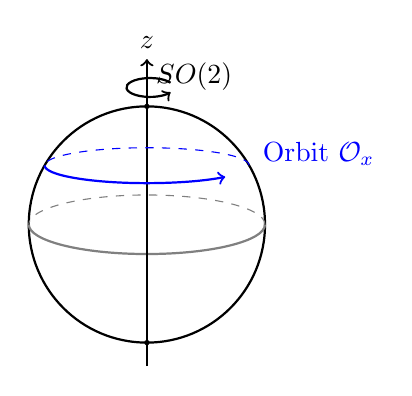
\begin{tikzpicture}[scale=1.5]
    % Draw the sphere outline
    \draw[thick] (0,0) circle (1);
    
    % Draw the equator (dashed back, solid front)
    \draw[gray, dashed] (1,0) arc (0:180:1 and 0.25);
    \draw[gray, thick] (-1,0) arc (180:360:1 and 0.25);
    
    % Draw the rotation axis (z-axis)
    \draw[thick, ->] (0,-1.2) -- (0,1.4) node[above] {$z$};
    
    % Label Poles
    \filldraw (0,1) circle (0.5pt) node[above right] {};
    \filldraw (0,-1) circle (0.5pt) node[below right] {};
    
    % Draw an Orbit (a circle of latitude)
    \draw[blue, dashed] ({sqrt(1-0.5^2)}, 0.5) arc (0:180:{sqrt(1-0.5^2)} and 0.15);
    \draw[blue, thick, ->] ({-sqrt(1-0.5^2)}, 0.5) arc (180:320:{sqrt(1-0.5^2)} and 0.15);
    \node[blue, right] at (0.9, 0.6) {Orbit $\mathcal{O}_x$};


    % Rotation Arrow at top
    \draw[->, thick] (0.2, 1.2) arc (30:330:0.2 and 0.08);
    \node at (0.4, 1.25) {$SO(2)$};

\end{tikzpicture}
\end{center}
\end{itemize}
\end{example}


\begin{definition}[Orbit and Stabilizer]
Let $G$ act on a set $X$. 
\begin{itemize}
\item The \textbf{orbit} of $x$, denoted by $G \cdot x$ or $\mathcal{O}_x$, is the subset of $X$ containing all elements that $x$ can be moved to by $G$:
\[ \mathcal{O}_x = \{ g \cdot x \mid g \in G \} \subseteq X \]

\item The \textbf{stabilizer} of $x$, denoted by $G_x$ or $\text{Stab}(x)$, is the set of elements in $G$ that fix $x$:
\[ G_x = \{ g \in G \mid g \cdot x = x \} \subseteq G \]
\end{itemize}
\end{definition}
\begin{example}
Note that for $x ,y \in X$,
$$x \sim y  \quad \Leftrightarrow \quad x, y \text{ are in the same orbit}$$
is an equivalence relation (Exercise). Therefore, the orbits form a partition of the set $X$. For instance, an orbit of $SO(2)$-action on $S^2$ in the above example is a {\it latitude line}
on the sphere (marked in blue). Obviously, lines of different latitudes give a partition of $S^2$.
\end{example}

As for the stabilizer, one can check that $G_x$ is always a subgroup of $G$ (Exercise). Therefore, if $G$ is finite, one always has
$$|G_x|\ |\ |G|$$
by Lagrange's theorem. Indeed, one has a more refined result in terms of the size of the orbit:
\begin{theorem}[Orbit-Stabilizer Theorem]
Let $G$ be a finite group acting on a set $X$. For any $x \in X$:
\[ |G| = |G_x| \cdot |\mathcal{O}_x| \]
Equivalently, the size of the orbit is the index of the stabilizer: $|\mathcal{O}_x| = [G : G_x]$.
\end{theorem}
\begin{proof}
To prove $|\mathcal{O}_x| = [G : G_x]$, we will construct a bijection $f$ between the set of all left cosets of $G_x$ in $G$ and the elements of the orbit $\mathcal{O}_x$. To do so,
let $G/G_x = \{ gG_x \mid g \in G \}$ be the set of left cosets, and define:
\[ f: G/G_x \to \mathcal{O}_x \quad \quad f(gG_x) := g \cdot x \]
\noindent{1. Well-defined:}
We must ensure that if two cosets are equal, their images are equal. Suppose $g_1G_x = g_2G_x$. Then $g_2^{-1}g_1 \in G_x$. By the definition of the stabilizer:
\begin{align*} (g_2^{-1}g_1) \cdot x &= x \\
 g_2 \cdot (g_2^{-1}g_1 \cdot x) &= g_2 \cdot x \\
(g_2 g_2^{-1} g_1) \cdot x &= g_2 \cdot x \\
 g_1 \cdot x &= g_2 \cdot x 
\end{align*}
Thus $f(g_1G_x) = f(g_2G_x)$, so $f$ is well-defined.

\noindent{2. Injective:}
Suppose $f(g_1G_x) = f(g_2G_x)$. Then:
\begin{align*} g_1 \cdot x &= g_2 \cdot x \\
g_2^{-1} \cdot (g_1 \cdot x) &= g_2^{-1} \cdot (g_2 \cdot x) \\
 (g_2^{-1}g_1) \cdot x &= e \cdot x = x \end{align*}
This implies $g_2^{-1}g_1 \in G_x\ \Leftrightarrow \ g_1G_x = g_2G_x$. Thus $f$ is injective.

\noindent{3. Surjective:}
By the definition of the orbit $\mathcal{O}_x$, any element $y \in \mathcal{O}_x$ is of the form $g \cdot x$ for some $g \in G$. Then $y = f(gG_x)$, so $f$ is surjective.

Since $f$ is a bijection, the number of elements in the orbit is equal to the number of left cosets:
\[ |\mathcal{O}_x| = |G/G_x| = [G : G_x] \]
By Lagrange's Theorem, we know that $[G : G_x] = \frac{|G|}{|G_x|}$. Therefore:
\[ |\mathcal{O}_x| = \frac{|G|}{|G_x|} \implies |G| = |\mathcal{O}_x| \cdot |G_x|. \]
\end{proof}


\begin{example}
Let $G$ be the group of rotational symmetries of the tetrahedron. Then $G$ defines an action on the $4$ faces of the tetrahedron. Suppose $x$ be a specific face of the tetrahedron, then:
\begin{itemize}
    \item There are $4$ faces, and any face can be rotated to any other face, so $|\mathcal{O}_x| = 4$.
    \item The rotations fixing face $x$ are the $3$ rotations (0, 120, 240 degrees) around the axis through the center of that face. So $|G_x| = 3$.    
\end{itemize}
By the Orbit-Stabilizer Theorem, one has $|G| = 4 \times 3 = 12$. But of course we already knew that the rotational symmetries of a tetrahedron is isomorphic to $A_4$, the alternating group. So we have re-confirmed that $|A_4| = 12$.
\end{example}

\begin{example}
Let $G$ be any finite group, and $X = G$. Then $G$ act on itself by conjugation: 
$$g \cdot x = gxg^{-1}.$$
In such a case:
\begin{itemize}
    \item The orbit $\mathcal{O}_x$ is the \textbf{conjugacy class} of $x$.
    \item The stabilizer $G_x$ is the \textbf{centralizer} $Z_G(x) := \{g \in G \mid gx = xg\}$.
\end{itemize}
By the orbit-stabilizer theorem, the size of a conjugacy class must divide the order of the group. Also, it can be computed by computing the centralizer group $Z_G(x)$ (see Homework). 
\end{example}

We end this section with Burnside's Lemma, which provides a way to count the number of distinct orbits in $X$ for any finite group action. 
\begin{theorem}[\textbf{Burnside's Lemma}]
Let $G$ be a finite group acting on a finite set $X$. Then the number of orbits, denoted $|X/G| := |\{\mathcal{O}_x\ |\ x \in X\}|$, is the average number of points fixed by the elements of $G$:
\[ |X/G| = \frac{1}{|G|} \sum_{g \in G} |X^g|, \]
where $X^g = \{ x \in X \mid g \cdot x = x \}$ be the set of points fixed by $g$.
\end{theorem}


\begin{proof}
Consider the set of all fixed pairs $S = \{ (g, x) \in G \times X \mid g \cdot x = x \}$. We will count the number of elements in $S$ in two different ways.

\noindent{Method 1: Summing over $G$}
For a fixed $g \in G$, the number of elements $x$ such that $(g, x) \in S$ is exactly $|X^g|$. Therefore:
\[ |S| = \sum_{g \in G} |X^g| \]

\noindent{Method 2: Summing over $X$}
For a fixed $x \in X$, the number of elements $g$ such that $(g, x) \in S$ is exactly the size of the stabilizer $G_x$. Therefore:
\[ |S| = \sum_{x \in X} |G_x| \]

Therefore, one has:
\[ \sum_{g \in G} |X^g| = \sum_{x \in X} |G_x| \]
Let $\Omega_1, \Omega_2, \dots, \Omega_k$ be the distinct orbits of $X$ (note that $k = |X/G|$). Then for any $x \in X$, $x \in \Omega_{i_x}$ for a unique $1 \leq i_x \leq k$. Therefore:
\[ \sum_{g \in G} |X^g|  = \sum_{x \in X} |G_x|= \sum_{x \in X} \frac{|G|}{|\mathcal{O}_x|} = |G| \sum_{x \in X} \frac{1}{|\mathcal{O}_x|}  = |G|\sum_{i=1}^k \sum_{x \in \Omega_i} \frac{1}{|\Omega_i|}  \quad \quad (*)\]
where the second $=$ comes from the Orbit-Stabilizer Theorem.

For any specific orbit $\Omega_i$, the inner sum $\sum_{x \in \Omega_i} \frac{1}{|\Omega_i|}$ is just adding the value $\frac{1}{|\Omega_i|}$ to itself $|\Omega_i|$ times:
\[ \sum_{x \in \Omega_i} \frac{1}{|\Omega_i|} = |\Omega_i| \cdot \frac{1}{|\Omega_i|} = 1 \]
Therefore, Equation $(*)$ reduces to
\[ \sum_{g \in G} |X^g| = |G|\sum_{i=1}^k 1 = |G| \cdot k = |G| \cdot |X/G| \]
and consequently \( |X/G| = \frac{1}{|G|} \sum_{g \in G} |X^g| \).
\end{proof}

\begin{example}
To see how many distinct ways can the vertices of a regular pentagon be colored using $3$ colors up rotations and reflections. For example, the following colorings are treated the same:

\newcommand{\drawcoloredpentagon}[7]{
    \begin{scope}[xshift=#1]
        % Draw edges
        \draw[thick, gray!40] (90:1) -- (162:1) -- (234:1) -- (306:1) -- (18:1) -- cycle;
        
        % Draw vertices with colors
        \filldraw[draw=black, thick, fill=#2] (90:1) circle (5pt);  % Top
        \filldraw[draw=black, thick, fill=#3] (162:1) circle (5pt); % Top-Left
        \filldraw[draw=black, thick, fill=#4] (234:1) circle (5pt); % Bottom-Left
        \filldraw[draw=black, thick, fill=#5] (306:1) circle (5pt); % Bottom-Right
        \filldraw[draw=black, thick, fill=#6] (18:1) circle (5pt);  % Top-Right
        
        % Label below
        \node at (0, -1.5) {\textbf{#7}};
    \end{scope}
}

\begin{center}
\begin{tikzpicture}[scale=1.2]

    % 1. Original Coloring
    % Pattern: Top=Red, Lefts=Blue, Rights=Green
    \drawcoloredpentagon{0cm}{red!80}{blue!80}{blue!80}{green!80}{green!80}{Original ($x$)}


    % 2. Rotated Coloring (Counter-Clockwise)
    % Red moves to Top-Left, Green moves to Top, etc.
    \drawcoloredpentagon{4cm}{green!80}{red!80}{blue!80}{blue!80}{green!80}{Rotated ($r \cdot x$)}

    % 3. Reflected Coloring (Vertical Reflection of the Original)
    % Red stays top, Blue/Green swap sides
    \drawcoloredpentagon{8cm}{red!80}{green!80}{green!80}{blue!80}{blue!80}{Reflected ($s \cdot x$)}
\end{tikzpicture}
\end{center}
since the second can be obtained from the first by rotation, and the third can be obtained from the first by reflection. 

Consider the action of $G = D_5$ on the set $X$ of 5 vertices each with three different possible colors. Therefore, there are
$$|X| = 3 \times 3 \times 3 \times 3 \times 3 = 3^5 = 243$$
elements in $X$. The three diagrams above are {\it in the same orbit} under our action. So we need to calculate $|X/G|$ -- the {\it distinct} orbits of $X$ under the action of $G$.

To do so, we need to calculate $X^g$ for each $g \in D_5$. A coloring $x \in X$ is fixed by $g \in D_5$ if all vertices in the same cycle of the permutation $g$ have the same color. If $g$ has $\ell$ cycles, there are $3^{\ell}$ fixed colorings. Therefore, one has
\begin{center}
\begin{tabular}{lllll}
\textbf{Element Type} & \textbf{No. of Elements} & \textbf{Cycle Structure} & \textbf{No. of Cycles} & $|X^g|$ \\ 
Identity & $1$ & $(1)(2)(3)(4)(5)$ & 5 & $3^5 = 243$ \\
Rotations & $4$ & $(1\,2\,3\,4\,5)$ & 1 & $3^1 = 3$ \\
Reflections & $5$ & $(1)(2\,5)(3\,4)$ & 3 & $3^3 = 27$ \\ 
\end{tabular}
\end{center}

Here is an example of the number of possible colorings for a reflection $s \in D_5$ along the axis passing through vertex $1$. Among all the possible $3^5$ colorings of the five vertices, the colorings such that $s$ fixes the coloring is of the form:
\begin{center}
\begin{tikzpicture}[scale=2]
    % Define coordinates for a regular pentagon
    \foreach \i in {1,2,3,4,5} {
        \coordinate (P\i) at ({90 + (\i-1)*72}:1);
    }

    % Draw the axis of reflection (through Vertex 1)
    \draw[dashed, red, thick] (0, 1.3) -- (0, -1.1) node[below] {};

    % Draw the edges of the pentagon
    \draw[thick, gray!50] (P1) -- (P2) -- (P3) -- (P4) -- (P5) -- cycle;

    % Draw the vertices with color coding based on cycles
    % Cycle 1: Vertex 1 (Fixed)
    \node[circle, draw, fill=blue!20, inner sep=3pt, thick] (V1) at (P1) {1};
    
    % Cycle 2: Vertices 2 and 5 (Swapped)
    \node[circle, draw, fill=green!20, inner sep=3pt, thick] (V2) at (P2) {2};
    \node[circle, draw, fill=green!20, inner sep=3pt, thick] (V5) at (P5) {5};
    
    % Cycle 3: Vertices 3 and 4 (Swapped)
    \node[circle, draw, fill=orange!20, inner sep=3pt, thick] (V3) at (P3) {3};
    \node[circle, draw, fill=orange!20, inner sep=3pt, thick] (V4) at (P4) {4};

    % Draw swap arrows to show the action
    \draw[<->, >=Stealth, thick, bend left=15] (V2) to node[above, font=\footnotesize] {} (V5);
    \draw[<->, >=Stealth, thick, bend right=15] (V3) to node[below, font=\footnotesize] {} (V4);

    % Legend/Explanation
    \node[anchor=west, align=left] at (1.2, 0) {
        \textbf{Cycles of the Reflection:} \\
        \textcolor{blue!70!black}{$\bullet$} \textbf{Cycle 1:} $\{1\}$  \\
        \textcolor{green!60!black}{$\bullet$} \textbf{Cycle 2:} $\{2, 5\}$  \\
        \textcolor{orange!80!black}{$\bullet$} \textbf{Cycle 3:} $\{3, 4\}$  \\
        \\[0.5em]
        Total independent choices of $X^s$: \\
        ${\color{blue} 3} \times {\color{green} 3} \times {\color{orange} 3} = 3^3$
    };
\end{tikzpicture}


\end{center}
By Burnside Lemma, the number of distinct colorings $|X/G|$ is given by:
\begin{align*} |X/G| = \frac{1}{|G|} \sum_{g \in G} |X^g|   = \frac{1}{10} \left( 1 \cdot 243 + 4 \cdot 3 + 5 \cdot 27 \right) = \frac{390}{10} = 39 \end{align*}

There are \textbf{39} distinct ways to color the vertices of a regular pentagon with 3 colors under dihedral symmetry.
\end{example}




\section{Normal Subgroups}
Recall that for a subgroup $H \le G$, the group $G$ can be partitioned into left cosets $G = \bigsqcup_i\ g_i H$ or right cosets $G = \bigsqcup_j\ H b_j$. A natural question is whether these partitions are identical—that is, whether $gH = Hg$ for all $g \in G$.

In general, the answer is no. Consider $G = S_3$ and $H = \langle (1\,2) \rangle$:
\begin{align*}
(1\,3)H &= \{ (1\,3), (1\,3)(1\,2) \} = \{ (1\,3), (1\,2\,3) \} \\
H(1\,3) &= \{ (1\,3), (1\,2)(1\,3) \} = \{ (1\,3), (1\,3\,2) \}
\end{align*}
Since $(1\,3)H \neq H(1\,3)$, we look for subgroups that satisfy this property.

\begin{definition}[Normal Subgroup]
A subgroup $H \le G$ is called a \textbf{normal subgroup} if $gH = Hg$ for all $g \in G$. We denote this by $H \triangleleft G$.
\end{definition}

\begin{example}
\begin{itemize}
    \item $A_n \triangleleft S_n$ for all $n$.
    \item If $G$ is abelian, then any subgroup $H \le G$ is normal. For any $g \in G$ and $h \in H$, $gh = hg$, so $gH = Hg$.
    \item $SL(n, \mathbb{R}) \triangleleft GL(n, \mathbb{R})$. Let $A \in GL(n, \mathbb{R})$ and $h \in SL(n, \mathbb{R})$. Then:
    \[ \det(A h A^{-1}) = \det(A) \det(h) \det(A)^{-1} = \det(A) \cdot 1 \cdot \frac{1}{\det(A)} = 1 \]
    Thus $A h A^{-1} \in SL(n, \mathbb{R})$, which implies $A H A^{-1} = H$, or $AH = HA$.
    \item If $H \le G$ and $[G:H] = 2$, then $H \triangleleft G$. In this case, $G$ is the disjoint union $H \sqcup gH$ and also $H \sqcup Hg$ for any $g \notin H$. It follows that $gH = G \setminus H = Hg$.
    \item The trivial subgroup $\{e\}$ and the group $G$ itself are always normal in $G$.
\end{itemize}
\end{example}

\begin{theorem}
Let $H \le G$ be a subgroup. The following are equivalent:
\begin{enumerate}
    \item[(i)] $H \triangleleft G$.
    \item[(ii)] $g h g^{-1} \in H$ for all $h \in H$ and $g \in G$.
    \item[(iii)] $g H g^{-1} = H$ for all $g \in G$.
\end{enumerate}
\end{theorem}

\begin{proof}
\begin{itemize}
    \item \textbf{(i) $\Rightarrow$ (ii):} By assumption, $gH = Hg$. Thus for any $h \in H$, $gh \in Hg$, so $gh = h'g$ for some $h' \in H$. Multiplying by $g^{-1}$ on the right gives $ghg^{-1} = h' \in H$.
    \item \textbf{(ii) $\Rightarrow$ (iii):} Condition (ii) implies $gHg^{-1} \subseteq H$ for all $g \in G$. Applying this to $g^{-1}$, we have $g^{-1}H(g^{-1})^{-1} \subseteq H \Rightarrow g^{-1}Hg \subseteq H$. Multiplying by $g$ on the left and $g^{-1}$ on the right gives $H \subseteq gHg^{-1}$. Thus $gHg^{-1} = H$.
    \item \textbf{(iii) $\Rightarrow$ (i):} If $gHg^{-1} = H$, then multiplying by $g$ on the right gives $(gHg^{-1})g = Hg$, so $gH = Hg$.
\end{itemize}
\end{proof}

\begin{corollary}
Let $\phi : G \to H$ be a group homomorphism. Then $\ker \phi \triangleleft G$.
\end{corollary}

\begin{proof}
Let $k \in \ker \phi$ and $g \in G$. We check the conjugation condition:
\[ \phi(g k g^{-1}) = \phi(g) \phi(k) \phi(g^{-1}) = \phi(g) e_H (\phi(g))^{-1} = \phi(g) (\phi(g))^{-1} = e_H \]
Since $\phi(g k g^{-1}) = e_H$, we have $g k g^{-1} \in \ker \phi$. By the previous theorem, $\ker \phi \triangleleft G$.
\end{proof}

\begin{example}
\begin{itemize}
    \item Consider $\det : GL(n, \mathbb{R}) \to \mathbb{R}^*$. Since $\ker(\det) = SL(n, \mathbb{R})$, it follows that $SL(n, \mathbb{R}) \triangleleft GL(n, \mathbb{R})$.
    \item Consider $\psi : S_n \to (\{ \pm 1 \}, \cdot)$ given by the parity of the permutation. Since $\ker \psi = A_n$, it follows that $A_n \triangleleft S_n$.
\end{itemize}
\end{example}

\section{Quotient Groups}
Let $H \triangleleft G$ be a normal subgroup. We want to define a group structure on the set of left cosets $G/H := \{ gH \mid g \in G \}$. To do this, we must ensure that the natural multiplication of cosets is independent of the choice of representative.

\begin{definition}[Quotient Group]
Let $G$ be a group and $H \triangleleft G$. The \textbf{quotient group} $G/H$ is the set of left cosets $\{ gH \mid g \in G \}$ equipped with the binary operation:
\[ (aH) * (bH) := (ab)H \]
\end{definition}

\begin{remark}
Since many different elements can represent the same coset (i.e., $a_1 H = a_2 H$ even if $a_1 \neq a_2$), we must verify that the operation is well-defined.
\end{remark}

\begin{proposition}
If $H \triangleleft G$, the operation $(aH) * (bH) = (ab)H$ is well-defined and makes $G/H$ into a group.
\end{proposition}

\begin{proof}
First, we show the operation is \textbf{well-defined}. Suppose $aH = a'H$ and $bH = b'H$. This implies $h_a := a^{-1} a' \in H$ and $h_b := b^{-1} b' \in H$. We compute:
\[ a'b' = (ah_a)(bh_b) = a b (b^{-1} h_a b) h_b \]
Since $H \triangleleft G$, the element $h_3 := b^{-1} h_a b$ is in $H$. Thus $a'b' = ab(h_3 h_b)$. Since $h_3 h_b \in H$, we have $a'b' \in (ab)H$, so $(a'b')H = (ab)H$.

Next, we check the \textbf{group axioms}:
\begin{enumerate}
    \item \textbf{Associativity:} $((aH)(bH))(cH) = (ab)H(cH) = (abc)H = aH(bc)H = (aH)((bH)(cH))$.
    \item \textbf{Identity:} The coset $eH = H$ serves as the identity since $(aH)(eH) = (ae)H = aH$.
    \item \textbf{Inverses:} The inverse of $aH$ is $a^{-1}H$, since $(aH)(a^{-1}H) = (aa^{-1})H = eH$.
\end{enumerate}
\end{proof}

\begin{example}
\begin{itemize}
    \item Let $G = \mathbb{Z}$ and $H = n\mathbb{Z}$. Since $G$ is abelian, $H$ is normal. The quotient group is:
    \[ G/H = \{ 0 + n\mathbb{Z}, 1 + n\mathbb{Z}, \dots, (n-1) + n\mathbb{Z} \} \]
    The operation is $(a + n\mathbb{Z}) + (b + n\mathbb{Z}) = (a+b) + n\mathbb{Z}$. This group is isomorphic to $(\mathbb{Z}_n, +)$. We often write $\mathbb{Z}/n\mathbb{Z} \cong \mathbb{Z}_n$.
    
    \item Since $A_n \triangleleft S_n$ and $|S_n/A_n| = |S_n|/|A_n| = 2$, the quotient group $S_n/A_n$ is a group of order 2. Any group of order 2 is isomorphic to $\mathbb{Z}_2$, so $S_n/A_n \cong \mathbb{Z}_2$.
    
    \item Since $SL(n, \mathbb{R}) \triangleleft GL(n, \mathbb{R})$, we can form the quotient group. Each coset is of the form:
    \[ A \cdot SL(n, \mathbb{R}) = \{ B \in GL(n, \mathbb{R}) \mid \det(B) = \det(A) \} \]
    The multiplication of cosets corresponds to the multiplication of their determinants: $\det(AB) = \det(A)\det(B)$. Thus, $GL(n, \mathbb{R})/SL(n, \mathbb{R}) \cong (\mathbb{R}^*, \times)$.
    
    \item Let $K = \{ e, (1\,2)(3\,4), (1\,3)(2\,4), (1\,4)(2\,3) \} \triangleleft S_4$. The quotient group $S_4/K$ has order $24/4 = 6$. It can be shown that $S_4/K \cong S_3$.
\end{itemize}
\end{example}

The construction of quotient groups is a powerful tool in group theory:
\begin{itemize}
    \item \textbf{Construction:} It allows us to construct new groups from existing ones (e.g., constructing $\mathbb{Z}_n$ from $\mathbb{Z}$).
    \item \textbf{Cauchy's Theorem:} If $G$ is a finite group and $p$ is a prime dividing $|G|$, then $G$ contains an element of order $p$. Quotient groups are used in the inductive proof of this theorem.
    \item \textbf{Classification:} They are essential for the classification of finite groups and understanding group extensions.
\end{itemize}

\begin{theorem}[First Isomorphism Theorem]
Let $\phi : G \to H$ be a group homomorphism. Then:
\[ G/\ker \phi \cong \mathrm{im }\ \phi \]
\end{theorem}

\begin{example}
\begin{itemize}
    \item Let $\phi : \mathbb{Z} \to \mathbb{Z}_n$ be defined by $\phi(a) = [a]_n$. Then $\ker \phi = n\mathbb{Z}$ and $\text{im } \phi = \mathbb{Z}_n$. By the First Isomorphism Theorem, $\mathbb{Z}/n\mathbb{Z} \cong \mathbb{Z}_n$.
    
    \item Let $\det : GL(n, \mathbb{R}) \to \mathbb{R}^*$ be the determinant map. Then $\ker(\det) = SL(n, \mathbb{R})$ and $\text{im}(\det) = \mathbb{R}^*$. Thus, $GL(n, \mathbb{R})/SL(n, \mathbb{R}) \cong \mathbb{R}^*$.
    
    \item Define $\phi : \mathbb{R} \to GL(2, \mathbb{R})$ by $\phi(x) = \begin{pmatrix} \cos x & -\sin x \\ \sin x & \cos x \end{pmatrix}$. This is a homomorphism where $\ker \phi = 2\pi\mathbb{Z}$ and the image is the special orthogonal group $SO(2)$. Hence, $\mathbb{R}/2\pi\mathbb{Z} \cong SO(2)$.
\end{itemize}
\end{example}

\begin{proof}
Define a map 
$$\Psi : G/\ker \phi \to \text{im } \phi$$ by $\Psi(g \ker \phi) := \phi(g)$. We verify the following properties:

\begin{enumerate}
    \item \textbf{$\Psi$ is well-defined and injective:} 
    Let $a, b \in G$. Then:
    \begin{align*}
    a \ker \phi = b \ker \phi &\iff a^{-1}b \in \ker \phi \\
    &\iff \phi(a^{-1}b) = e_H \\
    &\iff \phi(a)^{-1}\phi(b) = e_H \\
    &\iff \phi(a) = \phi(b) \\
    &\iff \Psi(a \ker \phi) = \Psi(b \ker \phi).
    \end{align*}
    Reading this from left to right shows $\Psi$ is well-defined; reading from right to left shows $\Psi$ is injective.

    \item \textbf{$\Psi$ is a homomorphism:}
    For any $a, b \in G$:
    \begin{align*}
    \Psi((a \ker \phi)(b \ker \phi)) &= \Psi(ab \ker \phi) \\
    &= \phi(ab) \\
    &= \phi(a)\phi(b) \\
    &= \Psi(a \ker \phi)\Psi(b \ker \phi).
    \end{align*}

    \item \textbf{$\Psi$ is surjective:}
    By definition, $\text{im } \phi = \{ \phi(g) \mid g \in G \}$. Since $\Psi(g \ker \phi) = \phi(g)$, every element in the image of $\phi$ has a preimage under $\Psi$.
\end{enumerate}
Since $\Psi$ is a bijective homomorphism, $G/\ker \phi \cong \text{im } \phi$.
\end{proof}

We end this section with the notion of simple groups. It will play a big role in the Galois theory course (MAT 5210).
\begin{definition}[Simple Group]
A group $G$ is called \textbf{simple} if $G$ has no normal subgroups other than the trivial subgroup $\{e\}$ and the group $G$ itself.
\end{definition}

\begin{remark}
The concept of simple groups is analogous to prime numbers in arithmetic. If a group $G$ is \textbf{not} simple, there exists a proper normal subgroup $N \triangleleft G$. This allows us to "decompose" $G$ into two smaller groups: the normal subgroup $N$ and the quotient group $G/N$, which can then be studied individually.

However, it is important to note that if $G$ is not simple with $N \lhd G$, it is \textbf{not} necessarily isomorphic to the direct product $N \times (G/N)$ (Exercise: Find one such example of $N$ and $G$).
\end{remark}

\begin{example}
\begin{itemize}
    \item The symmetric group $S_n$ is \textbf{not} simple for $n \geq 3$ because the alternating group $A_n$ is a proper normal subgroup ($A_n \triangleleft S_n$). We can analyze $S_n$ via $A_n$ and the quotient $S_n/A_n \cong \mathbb{Z}_2$, but $S_n \not\cong A_n \times \mathbb{Z}_2$ for $n \geq 3$.
    
    \item The alternating group $A_4$ is \textbf{not} simple because the Klein four-group 
    $$K = \{ e, (1\,2)(3\,4), (1\,3)(2\,4), (1\,4)(2\,3) \}$$ is a normal subgroup of $A_4$.
    
    \item The alternating group $A_n$ is simple for all $n \geq 5$ (Homework). This result is a cornerstone of Galois Theory, as it implies that there is no general formula using radicals to solve polynomial equations of degree 5 or higher.
\end{itemize}
\end{example}

\section{Fundamental Theorem of Finite Abelian Groups}
We will conclude our study of groups by giving a classification of all finite abelian groups up to isomorphism. Here are some initial observations:
\begin{enumerate}
    \item[(1)] $\mathbb{Z}_n \cong \mathbb{Z}/n\mathbb{Z}$ is abelian.
    \item[(2)] $G$ and $H$ are abelian if and only if $G \times H$ is abelian.
    \item[(3)] If $\gcd(m, n) = 1$, then $\mathbb{Z}_{mn} \cong \mathbb{Z}_m \times \mathbb{Z}_n$.
\end{enumerate}

\begin{theorem}
All finite abelian groups are of the form $G \cong \mathbb{Z}_{p_1^{a_1}} \times \dots \times \mathbb{Z}_{p_k^{a_k}}$ where $p_1 \le \dots \le p_k$ are primes and $a_i \in \mathbb{N} \setminus \{0\}$.
\end{theorem}

The proof consists of two main steps:
\begin{itemize}
    \item \textbf{Step 1:} If $|G| = q_1^{a_1} \dots q_r^{a_r}$ for distinct primes $q_i$, then $G \cong G_1 \times \dots \times G_r$ where $|G_i| = q_i^{a_i}$.
    \item \textbf{Step 2:} If $|G| = q^b$, then $G \cong \mathbb{Z}_{q^{b_1}} \times \dots \times \mathbb{Z}_{q^{b_r}}$ with $\sum b_j = b$.
\end{itemize}


\paragraph{Proof of Step 1}:
We only deal with the case when $r = 2$, and the general case follows by repeatedly using this case. 

Suppose $|G| = p^a q^b$ for distinct primes $p, q$. Let $m = p^a$ and $n = q^b$. We want to show $G \cong G_1 \times G_2$ with $|G_1| = m$ and $|G_2| = n$. Let 

$$G^m := \{ g^m \mid g \in G \}, \quad G^n := \{ g^n \mid g \in G \}.$$

\begin{itemize}
    \item \textbf{Claim 1 -} $G^m \cap G^n = \{e\}$: 
    
    Suppose $x \in G^m \cap G^n$. Then $x = g^m = h^n$. By Lagrange's Theorem, 
    $$x^n = g^{mn} = e \quad \quad x^m = h^{nm} = e.$$ 
    Since $\gcd(m, n) = 1$, there exist $\alpha, \beta \in \mathbb{Z}$ such that $\alpha m + \beta n = 1$ by Bezout's Theorem. Then 
    $$x^1 = x^{\alpha m + \beta n} = (x^m)^\alpha (x^n)^\beta = e \cdot e = e.$$
    
    \item \textbf{Claim 2 -} $\phi: G^m \times G^n \to G$ given by $\phi(g^m, h^n) := g^m(h^n)^{-1}$ is an isomorphism:
    
    Note that $\phi$ is a homomorphism because $G$ is abelian. For injectivity, if $g^m(h^n)^{-1} = e$, then $g^m = h^n \in G^m \cap G^n = \{e\}$, so $\ker \phi = \{(e, e)\}$. For surjectivity, for any $y \in G$, $y = y^{\alpha m + \beta n} = (y^\alpha)^m (y^\beta)^n = \phi((y^\alpha)^m, (y^{-\beta})^n)$.
    
    \item \textbf{Claim 3 -} $|G^m| = n$ and $|G^n| = m$:
    
    Suppose $q \mid |G^n|$. By Cauchy's Theorem (proved in Homework), there exists $x = g^n \in G^n$ of order $q$. By Bezout's Theorem, $\alpha q + \beta m = 1$ for some $\alpha, \beta \in \mathbb{Z}$. Then 
    $$x = x^{\alpha q + \beta m} = (x^q)^\alpha (x^m)^\beta = e \cdot (g^{nm})^\beta = e,$$ 
    contradicting $\text{ord}(x)=q$. Thus 
    $$\gcd(|G^n|, q) = 1 \Rightarrow |G^n| = p^r.$$
    Similarly $|G^m| = q^s$. Since $G^m \times G^n \cong G$, we have $p^r q^s = p^a q^b$, so $r=a, s=b$.
\end{itemize}

\paragraph{Proof of Step 2}:
Suppose $|G| = p^a$. By Lagrange's Theorem, for all $x \in G$:
\[ \text{ord}(x) = p^i \quad \text{for some } 0 \le i \le a. \]
Let $\mu \in G$ be an element with maximum order $\text{ord}(\mu) = p^m$ in $G$.

\begin{proposition}
Let $G$ be an abelian group with $|G| = p^a$. Suppose $\mu \in G$ has maximum order $\text{ord}(\mu) = p^m$ in $G$, then 
\[ G \cong \langle \mu \rangle \times K \cong \mathbb{Z}_{p^m} \times K. \]
\end{proposition}
Assuming the validity of the proposition, then one can reduce the study of $G$ into that of $K$, since $K$ is also abelian with $|K| = |G|/|\langle \mu \rangle| = p^{a-m}$. Then {\bf Step 2} follows by induction on power of $p$.


\begin{proof}[Proof of Proposition]
We proceed by induction on $|G| = p^a$. For the base case $a=1$, $|G| = p$ implies $G \cong \mathbb{Z}_p$, and the result holds with $K = \{e\}$. Assume the proposition holds for all abelian groups of order $p^r$ with $r < a$. 

Now let $|G| = p^a$ and let $\text{ord}(\mu) = p^m$ be maximal.
If $m=a$, then $\langle \mu \rangle = G$ and the result is trivial. Otherwise, if $m < a$, let $\nu \in G$ be a non-identity element not in $\langle \mu \rangle$ with the smallest possible order $p^k$.

\begin{itemize}
    \item \textbf{Claim 4 -} $\text{ord}(\nu) = p$: 
    
    Since $\text{ord}(\nu^p) < p^k$, by the minimality of $p^k$, we must have $\nu^p \in \langle \mu \rangle$, so $\nu^p = \mu^i$ for some $i \in \mathbb{Z}$. Then:
    \[ (\mu^i)^{p^{m-1}} = (\nu^p)^{p^{m-1}} = \nu^{p^m} = e \]
    since every element in $G$ has order $\le p^m$. This implies $\text{ord}(\mu^i) \mid p^{m-1}$, so $|\langle \mu^i \rangle| < p^m$, which means $\gcd(i, p^m) > 1$. Thus, $i = pj$ for some $j \in \mathbb{Z}$, and we have:
    \[ \nu^p = \mu^{pj}. \] 
    Let $c := \nu \mu^{-j}$. Then $c \notin \langle \mu \rangle$ and:
    \[ c^p = (\nu \mu^{-j})^p = \nu^p \mu^{-pj} = e. \]
    Since $\nu$ was chosen with the smallest order among elements not in $\langle \mu \rangle$, it follows that $\text{ord}(\nu) = p$.

    \item \textbf{Claim 5 -} $\langle \mu \rangle \cap \langle \nu \rangle = \{e\}$: 
    
    Let $\nu^l \in \langle \mu \rangle \cap \langle \nu \rangle$. Since $\text{ord}(\nu) = p$, we have $0 \le l < p$. If $l \neq 0$, then $\gcd(l, p) = 1$. By Bezout's Theorem, there exist $\alpha, \beta$ such that $\alpha l + \beta p = 1$. Then:
    \[ \nu = \nu^{\alpha l + \beta p} = (\nu^l)^\alpha (\nu^p)^\beta = (\nu^l)^\alpha \in \langle \mu \rangle \]
    which contradicts our choice of $\nu$. Thus $l=0$ and the intersection is trivial.

    \item \textbf{Claim 6 -} $\bar{\mu} \in \bar{G} := G/\langle \nu \rangle$ has order $p^m$: 
    
    Clearly $\bar{\mu}^{p^m} = e_{\bar{G}}$. Suppose $\text{ord}(\bar{\mu}) = p^u$ for some $u < m$. Then $\mu^{p^u} \langle \nu \rangle = e\langle \nu \rangle$, meaning $\mu^{p^u} \in \langle \nu \rangle$. By Claim 5:
    \[ \mu^{p^u} \in \langle \mu \rangle \cap \langle \nu \rangle = \{e\} \]
    which contradicts $\text{ord}(\mu) = p^m$. Thus, $\bar{\mu}$ retains the maximal order $p^m$ in $\bar{G}$.

    \item \textbf{Claim 7 -} The map $\pi|_K: K \to \bar{K}$ has $\ker(\pi|_K) = \langle \nu \rangle$: 
    
    Since $|\bar{G}| = p^{a-1}$, by the inductive hypothesis, there exists a subgroup $\bar{K} \le \bar{G}$ such that $\bar{G} \cong \langle \bar{\mu} \rangle \times \bar{K}$. Let $\pi: G \to \bar{G}$ be the natural projection and define $K := \pi^{-1}(\bar{K})$. Then:
    \[ x \in \ker(\pi|_K) \iff \pi(x) = e_{\bar{G}} \iff x \in \langle \nu \rangle. \]

    \item \textbf{Claim 8 -} $\langle \mu \rangle \cap K = \{e\}$ in $G$: 
    
    Let $\mu^i \in \langle \mu \rangle \cap K$. Then $\pi(\mu^i) = \bar{\mu}^i \in \bar{K}$. Since $\bar{G} = \langle \bar{\mu} \rangle \times \bar{K}$, every element is uniquely represented. Thus:
    \[ \bar{\mu}^i = e_{\bar{G}} \implies \mu^i \in \langle \nu \rangle. \]
    By Claim 5, $\mu^i \in \langle \mu \rangle \cap \langle \nu \rangle = \{e\}$.
\end{itemize}

Finally, consider the homomorphism $\theta: \langle \mu \rangle \times K \to G$ defined by $\theta(\mu^i, k) := \mu^i k$. By Claim 8, $\theta$ is injective. By Claim 7 and the First Isomorphism Theorem, the order of $K$ is:
\[ |K| = p \cdot |\bar{K}| = p \cdot \frac{|\bar{G}|}{p^m} = p \cdot \frac{p^{a-1}}{p^m} = p^{a-m}. \]
Thus, the order of the product group is:
\[ |\langle \mu \rangle \times K| = p^m \cdot p^{a-m} = p^a = |G|. \]
Therefore, $\theta$ is a bijection, and $G \cong \langle \mu \rangle \times K$.
\end{proof}

\begin{example}
Consider an abelian group $G$ with $|G| = 4$. By Lagrange's Theorem, the possible orders for elements in $G$ are 1, 2, and 4.
\begin{enumerate}
    \item[(i)] If $G$ contains an element $m$ of order 4, then $G = \langle m \rangle \cong \mathbb{Z}_4$.
    \item[(ii)] If every non-identity element of $G$ has order 2, let $m \in G$ be an element of order 2. By the previous proposition, $G \cong \langle m \rangle \times K \cong \mathbb{Z}_2 \times \mathbb{Z}_2$.
\end{enumerate}
\end{example}

\begin{corollary}
If $G$ is an abelian $p$-group with $|G| = p^a$, then 
\[ G \cong \mathbb{Z}_{p^{b_1}} \times \mathbb{Z}_{p^{b_2}} \times \dots \times \mathbb{Z}_{p^{b_\ell}} \]
where $\sum_{j=1}^{\ell} b_j = a$.
\end{corollary}
\begin{proof}
The proof follows by induction on $|G| = p^a$, using the proposition that $G \cong \mathbb{Z}_{p^m} \times K$ to repeatedly factor out cyclic components until the remaining group is trivial.
\end{proof}

\begin{example}
To classify all abelian groups of order $|G| = 360 = 2^3 \times 3^2 \times 5$:
\begin{itemize}
    \item \textbf{By Step 1:} The group decomposes into its Sylow $p$-subgroups:
    \[ G \cong G_8 \times G_9 \times G_5 \]
    where $|G_8| = 2^3$, $|G_9| = 3^2$, and $|G_5| = 5$.
    \item \textbf{By Step 2:} We find all possible structures for each $p$-group:
    \begin{itemize}
        \item $G_8$ can be $\mathbb{Z}_8$, $\mathbb{Z}_4 \times \mathbb{Z}_2$, or $\mathbb{Z}_2 \times \mathbb{Z}_2 \times \mathbb{Z}_2$.
        \item $G_9$ can be $\mathbb{Z}_9$ or $\mathbb{Z}_3 \times \mathbb{Z}_3$.
        \item $G_5$ can only be $\mathbb{Z}_5$.
    \end{itemize}
\end{itemize}
Thus, the total number of non-isomorphic abelian groups of order 360 is $3 \times 2 \times 1 = 6$. The possible structures are:
\[ G \cong \left\{ \begin{matrix} \mathbb{Z}_8 \\ \mathbb{Z}_4 \times \mathbb{Z}_2 \\ \mathbb{Z}_2^3 \end{matrix} \right\} \times \left\{ \begin{matrix} \mathbb{Z}_9 \\ \mathbb{Z}_3 \times \mathbb{Z}_3 \end{matrix} \right\} \times \mathbb{Z}_5 \]
\end{example}

\begin{corollary}[Smith Normal Form / Invariant Factors]
Every finite abelian group $G$ is isomorphic to a group of the form:
\[ G \cong \mathbb{Z}_{d_1} \times \mathbb{Z}_{d_2} \times \dots \times \mathbb{Z}_{d_k} \]
where each $d_i > 1$ is an integer and $d_i \mid d_{i+1}$ for all $i = 1, \dots, k-1$. 

Furthermore, this representation is unique: if $H \cong \mathbb{Z}_{e_1} \times \dots \times \mathbb{Z}_{e_\ell}$ with $e_i \mid e_{i+1}$, then $G \cong H$ if and only if $k = \ell$ and $d_i = e_i$ for all $i$.
\end{corollary}